\chapter{Results}
\label{chap:results}
We expect that the \gls{wdt} method will improve the statistics of
Serpent 2 calculations. With normal delta-tracking, virtual collisions
provide no statistical benefit, and are therefore an inefficient use
of computational resources. Virtual collisions that result in
absorption events do contribute to statistics when using
\gls{wdt}. Therefore, we expect an improvement in the results of a
Serpent 2 simulation. In this section, we will describe how
performance in Serpent 2 is quantified, describe the three test cases,
and the results of those test cases.

\section{Performance metrics}
\label{sec:fom}

\subsection{Figure of Merit}
\label{sec:fom}

Monte Carlo codes such as Serpent 2 run many batches of a single
simulation, calculating the mean of values of interest $\hat{x}$
across many runs. 
% does serpent use batches if fission isn't involved? 
% maybe define a batch?
% is this across many batches, or many simulated particles?
By the central limit theorem, we know that the
means across many simulations will form a normal distribution with
variance $\sigma^2(\hat{x})$. We are interested in reducing the
variance of the final value, which will provide more confidence in the
simulation results. In general, running the simulation more times will
reduce this variance at the cost of requiring more computation
time. The variance is proportional to the number of cycles $n$:
% Is this cycles, or number of particles? How is that related to batches?
\begin{equation}
\label{eq:variance}
  \sigma^2(\hat{x}) \propto \frac{1}{n}\:.
\end{equation}

Serpent 2 reports the standard deviation of the mean,
$\sigma(\hat{x})$, which is proportional to $n^{-1/2}$. The standard deviation
plotted against cycles is shown in Fig.~\ref{fig:error_convergence} on
a log-log plot. As expected, we see a linear evolution with a slope of
1/2 once enough cycles have been executed to give good statistical calculations.
\begin{figure}[hbtp]
  \centering
  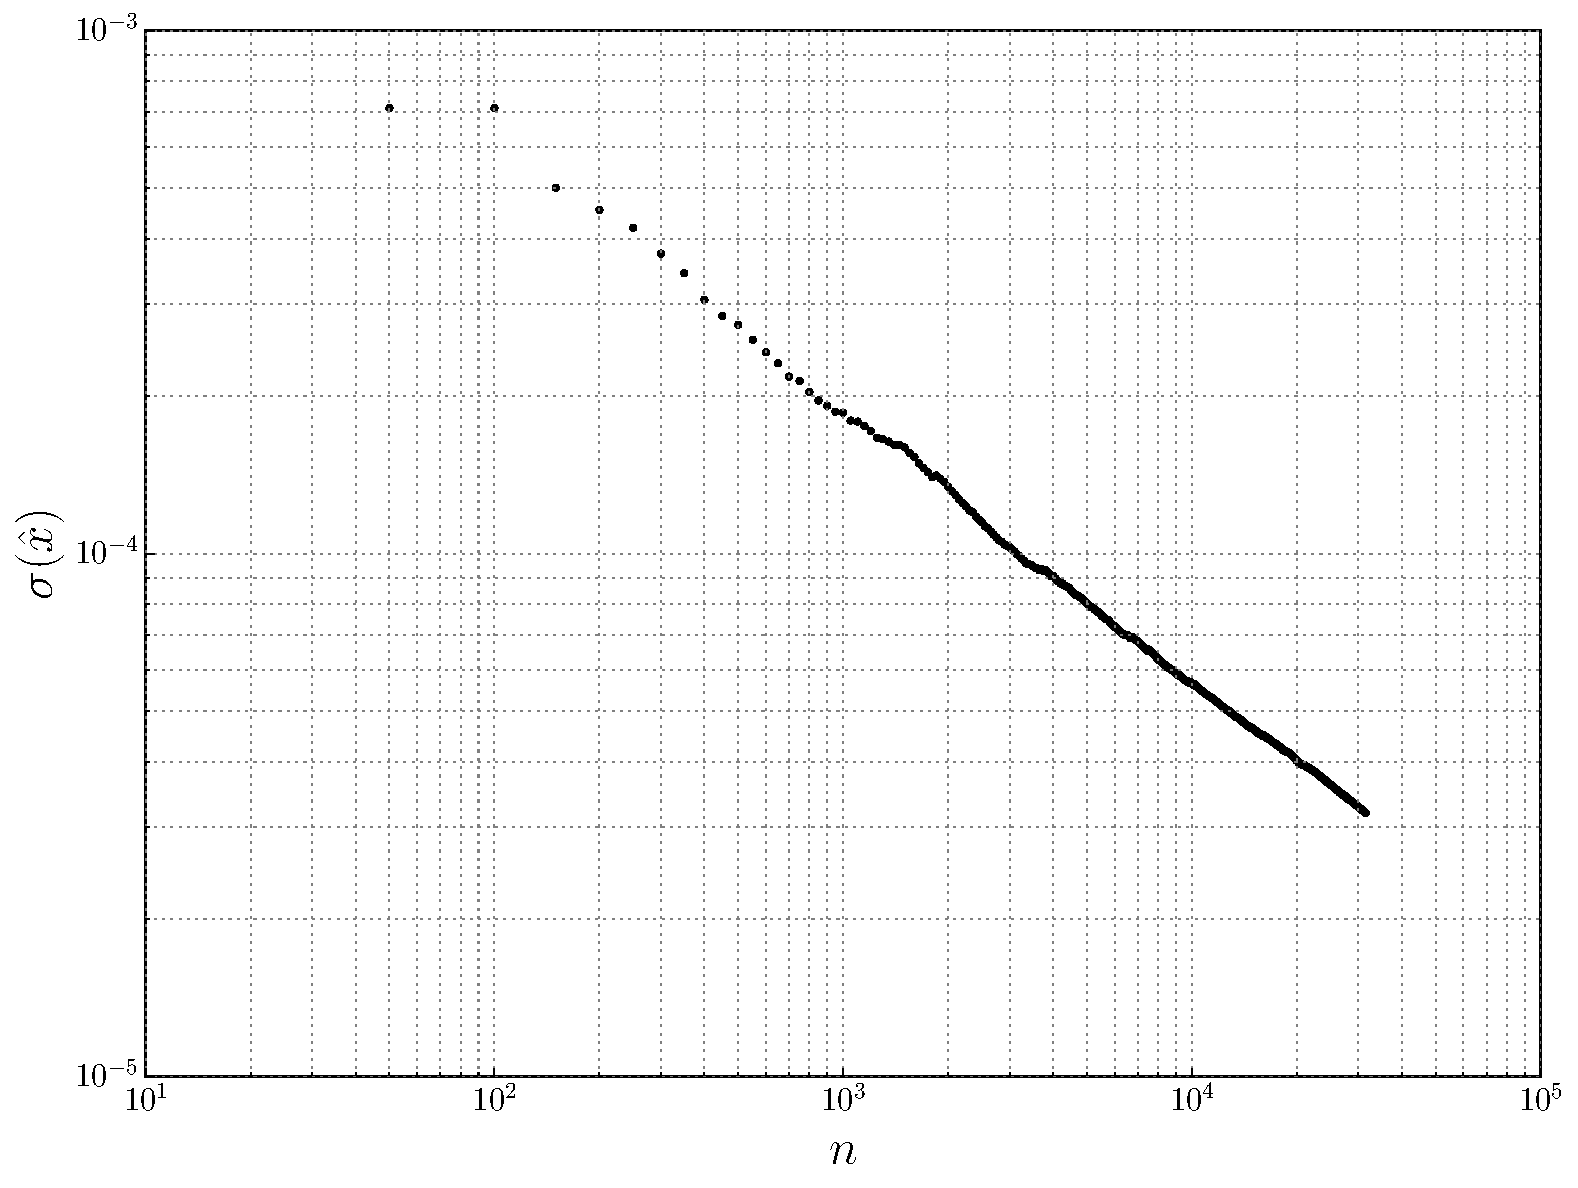
\includegraphics[scale=0.5]{images/error_convergence}
  \caption[Variance in $\phi_{\infty}$ for the fast-neutron group as a
    function of Serpent 2 cycle.]{Variance in $\phi_{\infty}$ for the fast-neutron group as a
    function of Serpent 2 cycle, with \gls{wdt} threshold of 0.2.}
  \label{fig:error_convergence}
\end{figure}
% you haven't defined \phi_{\infty}
We can always reduce the variance by running the simulation longer; a
% longer, or with more particles/cycles?
% I think this section needs a cleanup on precision of word choice about all of this. 
measure of our simulation quality, therefore, should be independent of
cycles. 

We establish a \gls{fom} that is independent of $n$.  The
standard \gls{fom} used by most simulations, described by Lewis and
Miller~\cite{lewis1993}, is shown in Eq.~\eqref{eq:fom}:
\begin{equation}
  \label{eq:fom}
  \mathrm{FOM} = \frac{1}{\sigma(\hat{x})^2T}\:,
\end{equation}
where $T$ is the runtime of the simulation and is proportional to the number
of cycles $T \propto n$. Plugging this and
Eq.~\eqref{eq:variance} into Eq.~\eqref{eq:fom} yields:
\begin{equation*}
  \mathrm{FOM} = \frac{1}{\sigma(\hat{x})^2T} =
  \frac{n}{C_1}\cdot\frac{1}{C_2\cdot n} = C_3\:,
\end{equation*}
where $C_1,C_2,C_3$ are constants. 

As we can see, we expect the
\gls{fom} to be a constant value, independent of the number of cycles
$n$.  A higher \gls{fom} indicates higher accuracy per computation
time, and therefore a more efficient algorithm. Serpent 2 collects
scores for each cycle (or batch of cycles) and outputs the sample mean
and standard deviation~\cite{VTT-R-00371-14}. This enables comparison of Serpent 2
running with and without \gls{wdt} to determine the efficiency of the
algorithm.

\subsection{Convergence}
\label{sec:convergence}

As discussed in the previous section, the \gls{fom} should be
independent of cycle number $n$. In reality, it takes enough cycles
for good statistics to develop for the \gls{fom} to converge to its
final value. As seen in Fig.~\ref{fig:fom_convergence}, the \gls{fom}
begins to converge around $1\times 10^4$ cycles in this example. Statistical
variations in the standard deviation seen in
Fig.~\ref{fig:error_convergence} are amplified by squaring and
inverting to calculate \gls{fom}. 
% why are we inverting and squaring the fom? how is that related to this plot?
It may take many cycles for the
\gls{fom} to converge to a single value. Therefore, we calculate an
average value using a selected number of the final data points.
\begin{figure}[hbtp]
  \centering
  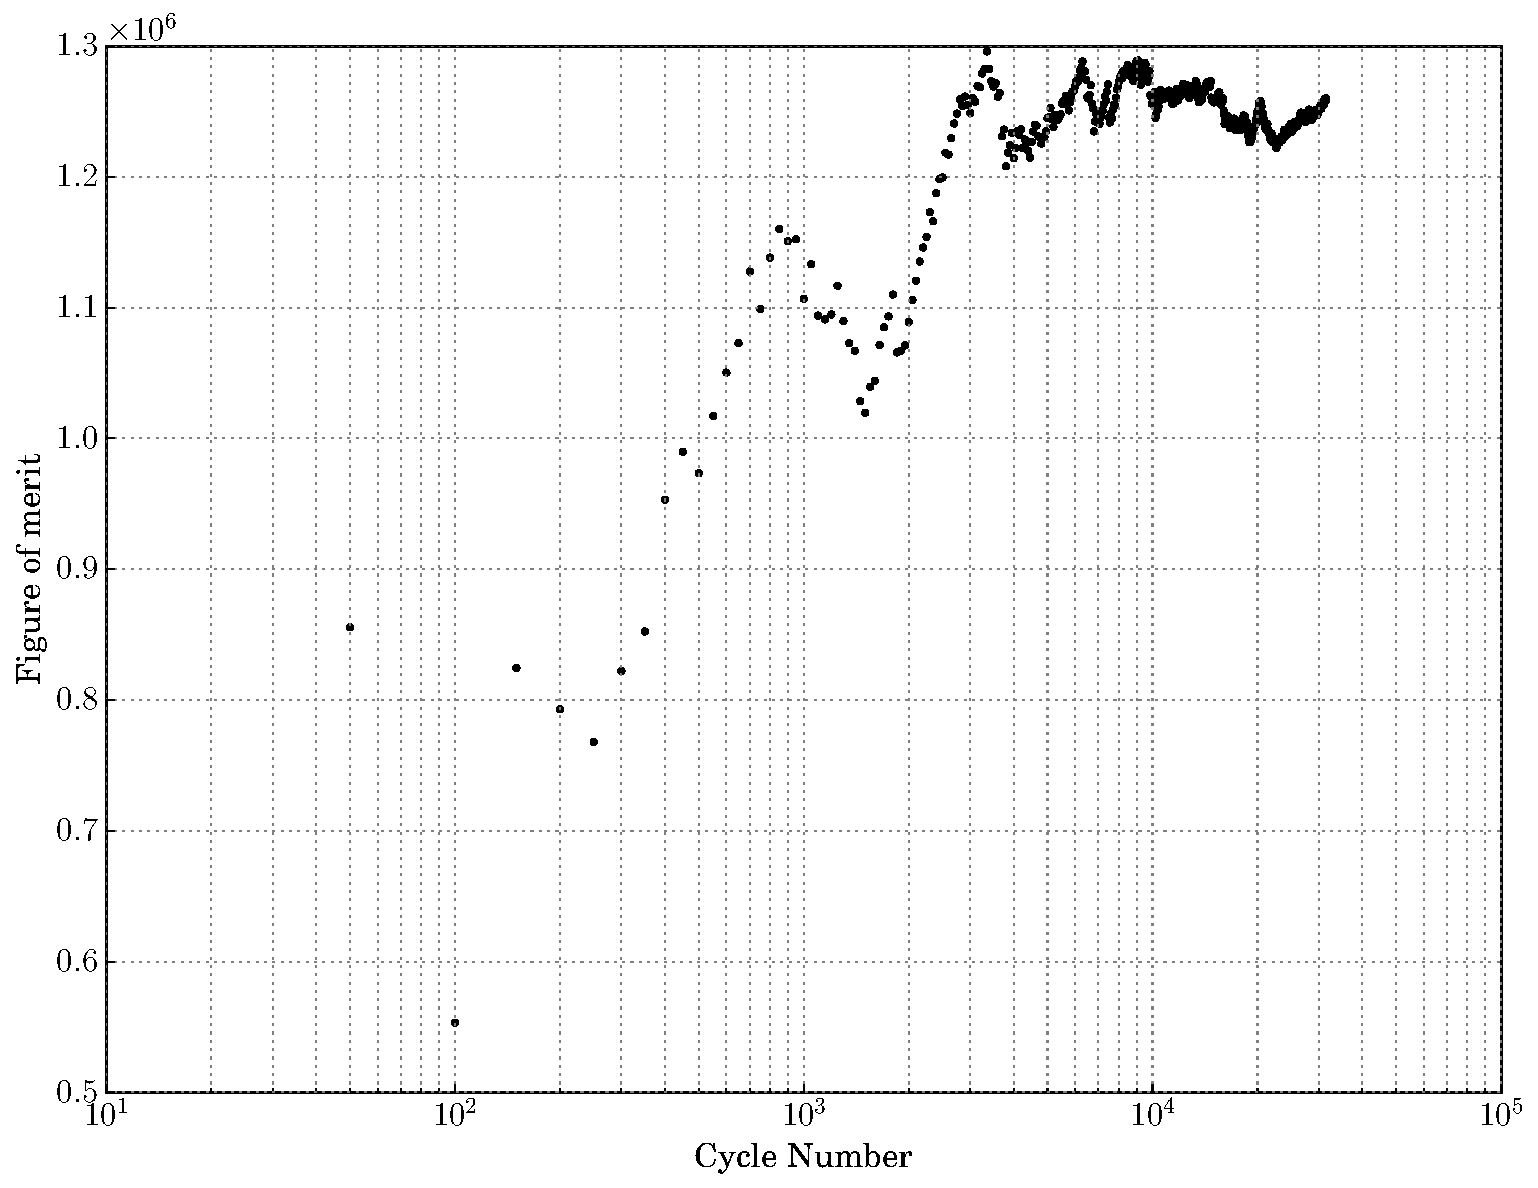
\includegraphics[scale=0.5]{images/fom_convergence_example}
  \caption[Figure of merit in $\phi_{\infty}$ for the fast-neutron group as a
    function of Serpent 2 cycle.]{Figure of merit in $\phi_{\infty}$ for the fast-neutron group as a
    function of Serpent 2 cycle, with \gls{wdt} threshold of 0.2.}
  \label{fig:fom_convergence}
\end{figure}

\section{Analysis Tools}
\label{sec:analysis}

Serpent 2 generates a single output file as the simulation runs. The
parameters of interest are overwritten as their mean value and
standard deviation are updated. This is sufficient to calculate the
final value of the \gls{fom}, which gives an indication of the quality
of the simulation. In addition to this, figures such as those shown in
Sec.~\ref{sec:fom} are useful to verify that the \gls{fom} has in fact
converged, and that the variance is reducing as expecting. Therefore,
in addition to changing the Serpent 2 source code to include the
\gls{wdt} method, it was modified to generate uniquely named output
files at the end of each batch. Processing these files enables us to
generate variance and FOM convergence graphs.

As seen in Fig.~\ref{fig:fom_convergence}, the final \gls{fom} is not
a single value, but may oscillate for a large number of
cycles. Therefore, we calculated an average \gls{fom} value for each
run, to allow comparison of runs without requiring a visual inspection
of each graph. To support processing the large amount of data, we
developed a python package, \verb|WDT_Analysis|.

\subsection{The \texttt{WDT\_Analysis} package}
\label{sec:wdt_analysis}

As described above, we modified the Serpent 2 source code to generate
uniquely named output files at various cycle values. The
\verb|WDT_Analysis| package leverages python's object oriented
% I'd maybe include a footnote with a link to the github, or something like that
% Whatever is the best way for someone to be able to find the package documentation.
programming structure to enable easy analysis of the data. We utilize
a module, \verb|fom|, to analyze the convergence of \gls{fom} across
many Serpent 2 output files. A summary
of each of the major objects used by the \verb|fom| module are outlined in
Table.~\ref{tab:wdt_analysis}.
\begin{table}[hbtp]
  \centering
  \caption{Object structure of the \texttt{WDT\_Analysis} package.\label{tab:wdt_analysis}}
  \begin{tabular}{ll} \toprule
   \textbf{Object} & \textbf{Description} \\ \midrule
    \verb|DataFile| & Contains all the data from a single Serpent 2
                      output file. \\
    \verb|Analyzer| & Contains all the \verb|DataFile| objects
                       from a run of Serpent 2. \\
    \verb|Comparator| & Compares the \gls{fom} convergence for one or
                        more \verb|Analyzer| objects. \\
    \bottomrule
  \end{tabular}
\end{table}
Detailed use of the package is provided in the package
documentation. Use of the package makes analysis of the \gls{fom}
convergence simple:
\begin{enumerate}
\item Run desired Serpent 2 simulations.
\item Place all output files from each desired run in separate directories
\item Initialize a \verb|Comparator| object, providing the directories
  and names for the datasets. While initializing, the
  \verb|Comparator| will:
  \begin{enumerate}
  \item Create a \verb|DataFile| object for each serpent output file.
  \item Collect the \verb|DataFile| objects from a single run into a single
    \verb|Analyzer|.
  \item Collect these \verb|Analyzer| objects into the
    \verb|Comparator|.
  \end{enumerate}
\item Use the \verb|compare| and \verb|plot| functions of the
  \verb|Comparator| object to observe the \gls{fom} convergence.
\end{enumerate}
We used this process to compare the \gls{fom} convergence for
different values of the \gls{wdt} threshold for three test cases.

\section{Parameters of Study}
\label{sec:parameters}
Each Serpent 2 simulation generates hundreds of output parameters that
describe all processes that occur during particle propagation. Finding
values where the \gls{wdt} method improves the \gls{fom} is a daunting
task. To focus our search, we identified three  quantities that
will be the focus of this research study. Further study into other
parameters may reveal further benefit or issues with the \gls{wdt}
method. The three parameters we selected are flux, 
total cross-section, and the scattering matrices for the
zeroth scattering moment. Each of the three test-cases have
reflective boundary conditions, so we will examine the infinite values for these
parameters.

The neutron flux quantifies the total distance traveled by all
neutrons in a volume per unit time. This is an important quantity, as
it is representative of the neutron population. A low variance is
desired in neutron flux, as it indicates that the uncertainty in the
neutron population in each energy group is well
understood.

The total cross-section quantifies the total interaction probability
for neutrons of that energy range. The zeroth scattering moment is a
matrix that quantifies scattering between the energy groups in the
problem, both upscattering and downscattering. A low variance is
desired in these parameters, as the goal of implementing this method
is to improve cross-section development for a highly scattering
medium, \gls{treat}.

A Serpent 2 simulation was run for each of the three test cases using
values of the \gls{wdt} threshold ($t_\mathrm{wdt}$) from 0.1 to unity in increments of
0.1, maintaining a value of $(1-c) = 0.1$, as described in
Fig.~\ref{fig:ray_wdt}. To determine the effectiveness of \gls{wdt},
we compared the final average \gls{fom} for each value of
$t_{\mathrm{wdt}}$ to the final average \gls{fom} with no \gls{wdt}:
\begin{equation*}
  R(t_{\mathrm{wdt}}) =
  \frac{\overline{\mathrm{FOM}}(t_\mathrm{wdt})}{\overline{\mathrm{FOM}}_0}
\end{equation*}
Where $\overline{\mathrm{FOM}}_0 =
\overline{\mathrm{FOM}}(0.1)$ is
the average \gls{fom} with no \gls{wdt}. Increasing values of
$t_{\mathrm{wdt}}$ leads to increasing amount of \gls{wdt} over
regular delta-tracking. The parameters for the rouletting scheme are
kept constant, with a weight cutoff of $w = 0.1$ and probability of
rouletting $P_{\mathrm{kill}} = 0.5$.

\subsection{Test Cases}
\label{sec:test_cases}

Three test cases were selected to test the \gls{fom} values for the
\gls{wdt} method. These are a \gls{pwr} pin cell, a fast reactor pin
cell, and a homogenous fuel element based on the composition of the
\gls{treat} fuel elements at the \gls{inl}. All test cases were run on
the Abacus server at UC Berkeley, the specifications of the server are
shown in Tab.~\ref{tab:abacus}.
\begin{table}[hbtp]
  \centering
  \caption{Abacus server specifications}
  \begin{tabular}{ll}
    \toprule
    \textrm{Parameter} & \textrm{Specification} \\ \midrule
    Processor & 2 x TenCore Intel Xeon Processor E5­2687W v3 3.10GHz
                 25MB Cache \\
    RAM & 16 x 16GB PC4­17000 2133MHz DDR4 \\
    Hard drive & 2 x 800GB Intel SATA 6.0Gb/s Solid State Drive
          \\ \bottomrule
  \end{tabular}
  \label{tab:abacus}
\end{table}

\section{\Acrlong{pwr} pin cell}
\label{sec:pwr}
The \gls{pwr} pin cell was chosen from the Serpent 2 validation input
files provided on the \gls{vtt} Serpent
webpage~\cite{serpent_web}. The geometry and physical parameters are
shown in Fig.~\ref{fig:pwr}. The fuel is a 2.68 w/o enriched UO$_2$
mixture, with Zircalloy cladding, light water moderation, and
reflective boundary conditions. We ran the simulation with two energy
groups with the group boundary at 0.625 eV.
\begin{figure}[hbtp]
  \centering
  \begin{tabular}{cc}
  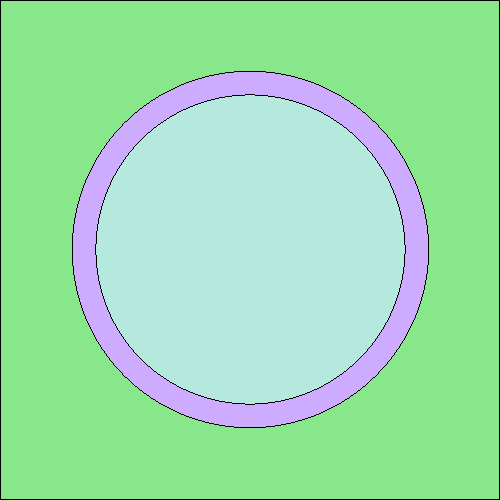
\includegraphics[scale=0.5]{images/results/pwr_geom1} \\
\begin{tabular}{@{}lr@{}}
\toprule
\textbf{Parameter}     & \textbf{Value (cm)} \\ \midrule
Fuel radius     & 0.412          \\
Cladding radius & 0.475          \\
Pitch              & 1.33          \\ \bottomrule
\end{tabular}
  \end{tabular}
  \caption[Pressurized water reactor geometry and physical
  parameters.]{Pressurized water reactor geometry and physical
    parameters. The fuel is shown in light blue, the cladding in
    purple and the coolant is green.}
  \label{fig:pwr}
\end{figure}
\subsection{Infinite Flux}
A summary of the \gls{fom} ratio,
$\overline{\mathrm{FOM}}(t_{\mathrm{wdt}})$, for the \gls{pwr} pin
cell for infinite flux ($\phi_{\infty}$) is shown in Tab.~\ref{tab:pwr_inf_flx} and
shown graphically in Fig.~\ref{fig:pwr_inf_flx}.
\begin{table}[hbtp]
  \centering
  \caption[$\overline{\mathrm{FOM}}$ and ratio for
    the \acrshort{pwr} pin cell infinite flux.]{$\overline{\mathrm{FOM}}$ as a function of
    $t_{\mathrm{wdt}}$ and the ratio of values to the base case for
    the \gls{pwr} pin cell infinite flux.}
  \begin{tabular}{cc} Fast group ($E > 0.0625$) & Slow group \\
\begin{tabular}{lrr}
\toprule
$t_{\mathrm{wdt}}$ &                   $\overline{\mathrm{FOM}}$ & Ratio\\
\midrule
 0.1 & 1.240281$\times 10^{6}$ & 1.000000 \\
 0.2 & 1.257046$\times 10^{6}$ & 1.013517 \\
 0.3 & 1.262320$\times 10^{6}$ & 1.017769 \\
 0.4 & 1.302585$\times 10^{6}$ & 1.050233 \\
 0.5 & 1.268738$\times 10^{6}$ & 1.022944 \\
 0.6 & 1.304854$\times 10^{6}$ & 1.052063 \\
 0.7 & 1.311428$\times 10^{6}$ & 1.057364 \\
 0.8 & 1.296513$\times 10^{6}$ & 1.045338 \\
 0.9 & 1.306470$\times 10^{6}$ & 1.053366 \\
 1.0 & 1.302047$\times 10^{6}$ & 1.049800 \\
\bottomrule
\end{tabular} &
\begin{tabular}{lrr}
\toprule
$t_{\mathrm{wdt}}$ &                   $\overline{\mathrm{FOM}}$ &
                                                                   Ratio\\
\midrule
 0.1 & 1.283594$\times 10^{6}$ & 1.000000 \\
 0.2 & 1.305878$\times 10^{6}$ & 1.017360 \\
 0.3 & 1.335006$\times 10^{6}$ & 1.040053 \\
 0.4 & 1.309221$\times 10^{6}$ & 1.019965 \\
 0.5 & 1.322382$\times 10^{6}$ & 1.030218 \\
 0.6 & 1.321435$\times 10^{6}$ & 1.029481 \\
 0.7 & 1.283419$\times 10^{6}$ & 0.999863 \\
 0.8 & 1.304767$\times 10^{6}$ & 1.016495 \\
 0.9 & 1.339323$\times 10^{6}$ & 1.043416 \\
 1.0 & 1.360193$\times 10^{6}$ & 1.059675 \\
\bottomrule
\end{tabular}
  \end{tabular}

  \label{tab:pwr_inf_flx}
\end{table}
\begin{figure}[hbtp]
  \centering
  \begin{tabular}{c}
  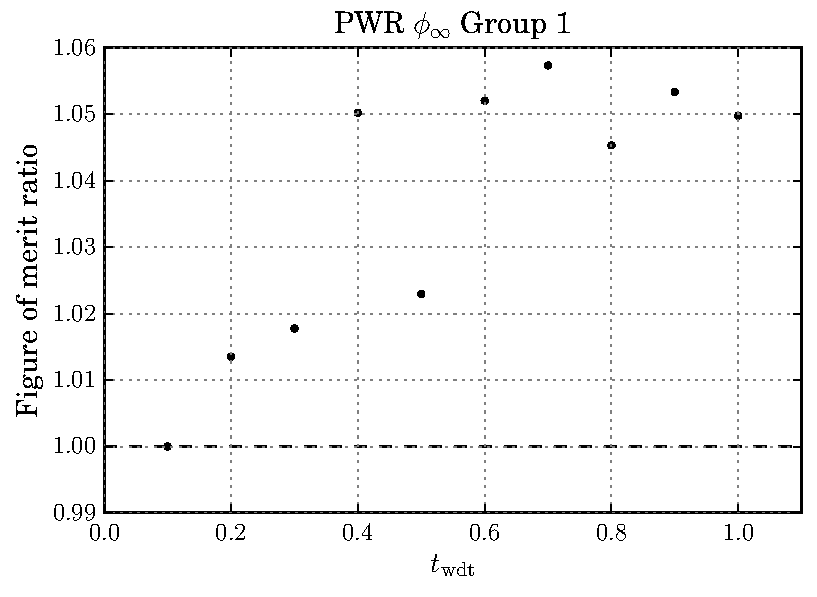
\includegraphics[scale=0.9]{images/results/pwr_inf_flx_grp_1} \\
    (a) Group 1\\
  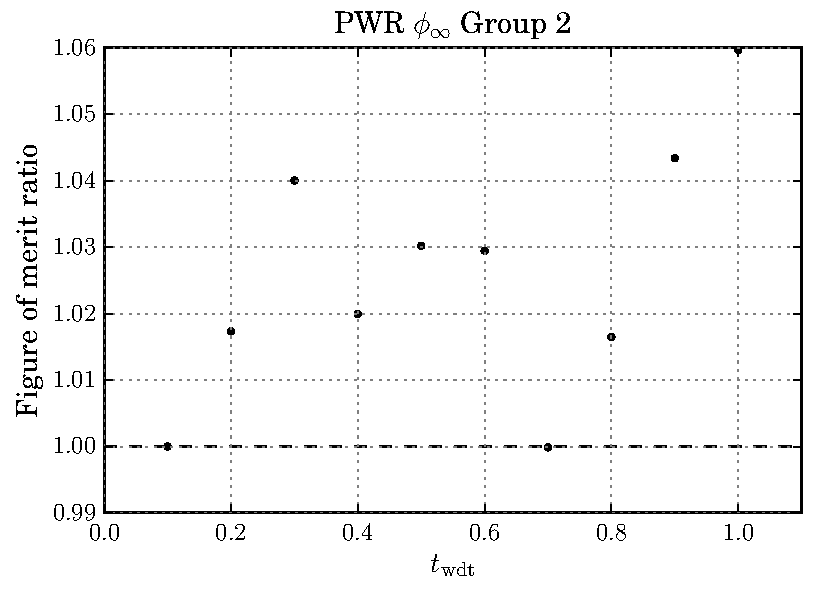
\includegraphics[scale=0.9]{images/results/pwr_inf_flx_grp_2} \\
    (b) Group 2
  \end{tabular}
  \caption[Figure of merit ratio of the infinite flux for the
  PWR]{Figure of merit ratio of the infinite flux for the PWR vs the
    \gls{wdt} threshold for the (a) high and (b) low energy
    groups. The group boundary is at $0.0625$ eV. \gls{fom} is
    calculated using the last 20 data points.}
  \label{fig:pwr_inf_flx}
\end{figure}

These ratios were calculated using the final 20 data points for each
series, then comparing to the base case. For the fast group, \gls{wdt} threshold values
of 0.6 and higher return a consistently higher \gls{fom} ratio. This
behavior is not observed in the slow group \gls{fom} ratio.

\subsection{Infinite Total Cross-section}
\label{sec:pwr_inf_total}
A summary of the \gls{fom} ratio,
$\overline{\mathrm{FOM}}(t_{\mathrm{wdt}})$, for the \gls{pwr} pin
cell for infinite total cross-section ($\Sigma_{t,
  \infty}$) is shown in Tab.~\ref{tab:pwr_inf_tot} and shown
graphically in Fig.~\ref{fig:pwr_inf_tot}. The \gls{fom} ratio for the
fast group when using \gls{wdt} is always less than unity. The
value has a similar behavior to the fast group infinite flux \gls{fom}
ratio, but inverted. The slow group shows consistent improvement, but
with no meaningful trend. the peak improvement occurs with full
\gls{wdt}, $t_{\mathrm{wdt}} = 1.0$, as with the infinite flux.

\begin{table}[hbtp]
  \centering
  \caption[$\overline{\mathrm{FOM}}$ and ratio for
  the \acrshort{pwr} pin cell infinite total cross-section.]{$\overline{\mathrm{FOM}}$ as a function of
    $t_{\mathrm{wdt}}$ and the ratio of values to the base case for
    the \gls{pwr} pin cell infinite total cross-section.}
  \begin{tabular}{cc} Fast group ($E > 0.0625$) & Slow group \\
\begin{tabular}{lrr}
\toprule
$t_{\mathrm{wdt}}$ &                   $\overline{\mathrm{FOM}}$ & Ratio\\
\midrule
 0.1 & 1.467242$\times 10^{7}$ & 1.000000 \\
 0.2 & 1.407526$\times 10^{7}$ & 0.959300 \\
 0.3 & 1.404113$\times 10^{7}$ & 0.956974 \\
 0.4 & 1.419632$\times 10^{7}$ & 0.967552 \\
 0.5 & 1.155054$\times 10^{7}$ & 0.787228 \\
 0.6 & 1.181301$\times 10^{7}$ & 0.805117 \\
 0.7 & 1.191133$\times 10^{7}$ & 0.811818 \\
 0.8 & 1.188149$\times 10^{7}$ & 0.809784 \\
 0.9 & 1.212526$\times 10^{7}$ & 0.826398 \\
 1.0 & 1.199368$\times 10^{7}$ & 0.817430 \\
\bottomrule
\end{tabular} &
\begin{tabular}{lrr}
\toprule
$t_{\mathrm{wdt}}$ &                   $\overline{\mathrm{FOM}}$ &
                                                                   Ratio\\
\midrule
 0.1 & 8.065829$\times 10^{6}$ & 1.000000 \\
 0.2 & 8.154616$\times 10^{6}$ & 1.011008 \\
 0.3 & 8.231395$\times 10^{6}$ & 1.020527 \\
 0.4 & 8.172302$\times 10^{6}$ & 1.013200 \\
 0.5 & 8.221818$\times 10^{6}$ & 1.019339 \\
 0.6 & 8.270724$\times 10^{6}$ & 1.025403 \\
 0.7 & 8.280600$\times 10^{6}$ & 1.026627 \\
 0.8 & 8.273215$\times 10^{6}$ & 1.025712 \\
 0.9 & 8.114104$\times 10^{6}$ & 1.005985 \\
 1.0 & 8.670363$\times 10^{6}$ & 1.074950 \\
\bottomrule
\end{tabular}
  \end{tabular}
  \label{tab:pwr_inf_tot}
\end{table}
\begin{figure}[hbtp]
  \centering
  \begin{tabular}{c}
  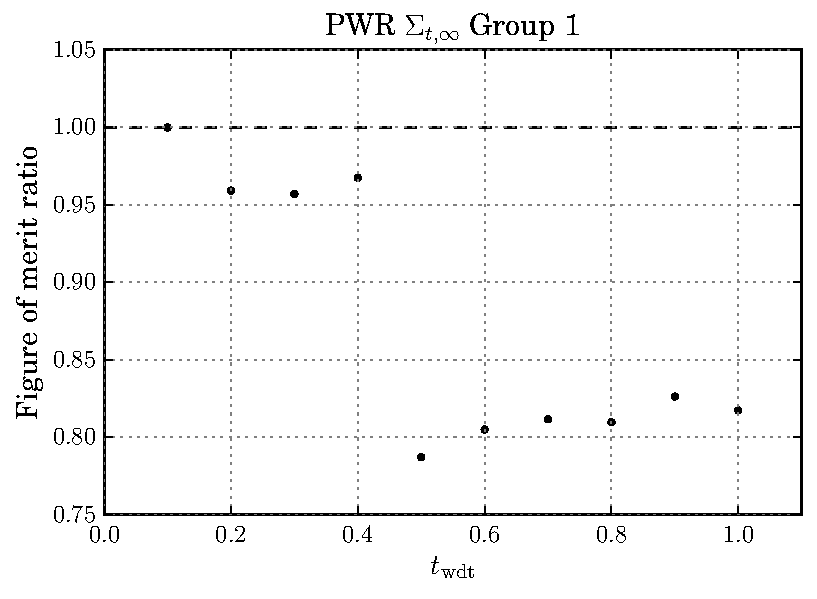
\includegraphics[scale=0.9]{images/results/pwr_inf_tot_grp_1} \\
    (a) \\
  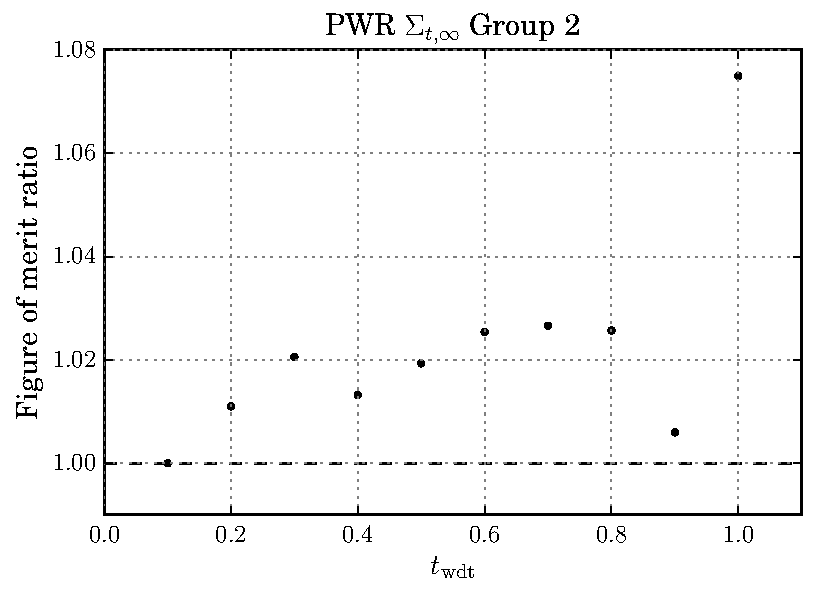
\includegraphics[scale=0.9]{images/results/pwr_inf_tot_grp_2} \\
    (b) 
  \end{tabular}
  \caption[Figure of merit ratio of the infinite total cross-section for the
  PWR]{Figure of merit ratio of the infinite total cross-section for the PWR vs the
    \gls{wdt} threshold for the (a) high and (b) low energy
    groups. The group boundary is at $0.0625$ eV. \gls{fom} is
    calculated using the last 20 data points.}
  \label{fig:pwr_inf_tot}
\end{figure}

\subsection{Scattering Matrices}
\label{sec:pwr_inf_total}

For the two-group case, the scattering matrices for the zeroth
moments $S_0$ is $2 \times 2$. A summary of the \gls{fom} ratio
for the zeroth moment $S_0$ is shown in Table~\ref{tab:pwr_inf_sp0}. The
tables are for the entry in row $g$ and column $g'$, which represents
scattering from group $g'$ into group $g$, indicated as $g' \to g$.

The \gls{wdt} method under-performs in most cases, except the
inscattering cross-section for the thermal group. 

\begin{table}[hbtp]
  \centering
  \caption[$\overline{\mathrm{FOM}}$ and ratio for
  the \acrshort{pwr} pin cell infinite $S_0$ scattering matrix.]{$\overline{\mathrm{FOM}}$ as a function of
    $t_{\mathrm{wdt}}$ and the ratio of values to the base case for
    the \gls{pwr} pin cell infinite $S_0$ scattering matrix}

  \begin{tabular}{cc} $\Sigma_{1\to 1}$ & $\Sigma_{2 \to 1}$ \\
\begin{tabular}{lrr}
\toprule
$t_{\mathrm{wdt}}$ &                   $\overline{\mathrm{FOM}}$ & Ratio\\
\midrule
 0.1 & 1.422641$\times 10^{7}$ & 1.000000 \\
 0.2 & 1.358990$\times 10^{7}$ & 0.955258 \\
 0.3 & 1.359954$\times 10^{7}$ & 0.955936 \\
 0.4 & 1.378010$\times 10^{7}$ & 0.968628 \\
 0.5 & 1.135270$\times 10^{7}$ & 0.798002 \\
 0.6 & 1.174407$\times 10^{7}$ & 0.825511 \\
 0.7 & 1.193568$\times 10^{7}$ & 0.838981 \\
 0.8 & 1.191534$\times 10^{7}$ & 0.837551 \\
 0.9 & 1.220204$\times 10^{7}$ & 0.857703 \\
 1.0 & 1.211019$\times 10^{7}$ & 0.851247 \\
\bottomrule
\end{tabular} &
\begin{tabular}{lrr}
\toprule
$t_{\mathrm{wdt}}$ &                   $\overline{\mathrm{FOM}}$ &
                                                                   Ratio\\
\midrule
 0.1 & 1.395679$\times 10^{6}$ & 1.000000 \\
 0.2 & 1.366134$\times 10^{6}$ & 0.978831 \\
 0.3 & 1.401562$\times 10^{6}$ & 1.004215 \\
 0.4 & 1.402313$\times 10^{6}$ & 1.004753 \\
 0.5 & 1.190960$\times 10^{6}$ & 0.853319 \\
 0.6 & 1.199284$\times 10^{6}$ & 0.859284 \\
 0.7 & 1.199826$\times 10^{6}$ & 0.859672 \\
 0.8 & 1.190166$\times 10^{6}$ & 0.852750 \\
 0.9 & 1.189501$\times 10^{6}$ & 0.852274 \\
 1.0 & 1.180054$\times 10^{6}$ & 0.845505 \\
\bottomrule
\end{tabular} \\

$\Sigma_{1\to 2}$ & $\Sigma_{2 \to 2}$ \\
\begin{tabular}{lrr}
\toprule
$t_{\mathrm{wdt}}$ &                   $\overline{\mathrm{FOM}}$ & Ratio\\
\midrule
 0.1 & 9.700866$\times 10^{3}$ & 1.000000 \\
 0.2 & 9.397108$\times 10^{3}$ & 0.968688 \\
 0.3 & 9.525420$\times 10^{3}$ & 0.981914 \\
 0.4 & 9.411723$\times 10^{3}$ & 0.970194 \\
 0.5 & 7.684674$\times 10^{3}$ & 0.792164 \\
 0.6 & 7.966642$\times 10^{3}$ & 0.821230 \\
 0.7 & 7.659128$\times 10^{3}$ & 0.789530 \\
 0.8 & 7.866229$\times 10^{3}$ & 0.810879 \\
 0.9 & 7.728249$\times 10^{3}$ & 0.796656 \\
 1.0 & 7.551567$\times 10^{3}$ & 0.778443 \\
\bottomrule
\end{tabular} &
\begin{tabular}{lrr}
\toprule
$t_{\mathrm{wdt}}$ &                   $\overline{\mathrm{FOM}}$ &
                                                                   Ratio\\
\midrule
 0.1 & 1.395679$\times 10^{6}$ & 1.000000 \\
 0.2 & 1.366134$\times 10^{6}$ & 0.978831 \\
 0.3 & 1.401562$\times 10^{6}$ & 1.004215 \\
 0.4 & 1.402313$\times 10^{6}$ & 1.004753 \\
 0.5 & 1.190960$\times 10^{6}$ & 0.853319 \\
 0.6 & 1.199284$\times 10^{6}$ & 0.859284 \\
 0.7 & 1.199826$\times 10^{6}$ & 0.859672 \\
 0.8 & 1.190166$\times 10^{6}$ & 0.852750 \\
 0.9 & 1.189501$\times 10^{6}$ & 0.852274 \\
 1.0 & 1.180054$\times 10^{6}$ & 0.845505 \\
\bottomrule
\end{tabular}
  \end{tabular}
  \label{tab:pwr_inf_sp0}
\end{table}

% % ==================== PWR S_1 Table

% \begin{table}[hbtp]
%   \centering
%   \caption[$\overline{\mathrm{FOM}}$ and ratio for
%   the \acrshort{pwr} pin cell infinite $S_1$ scattering matrix.]{$\overline{\mathrm{FOM}}$ as a function of
%     $t_{\mathrm{wdt}}$ and the ratio of values to the base case for
%     the \gls{pwr} pin cell infinite $S_1$ scattering matrix}
%   \begin{tabular}{cc} $\Sigma_{1\to 1}$ & $\Sigma_{2 \to 1}$ \\
% \begin{tabular}{lrr}
% \toprule
% $t_{\mathrm{wdt}}$ &                   $\overline{\mathrm{FOM}}$ & Ratio\\
% \midrule
%  0.1 & 6.050967$\times 10^{6}$ & 1.000000 \\
%  0.2 & 5.751850$\times 10^{6}$ & 0.950567 \\
%  0.3 & 5.622341$\times 10^{6}$ & 0.929164 \\
%  0.4 & 5.716568$\times 10^{6}$ & 0.944736 \\
%  0.5 & 4.676774$\times 10^{6}$ & 0.772897 \\
%  0.6 & 4.697950$\times 10^{6}$ & 0.776397 \\
%  0.7 & 4.732003$\times 10^{6}$ & 0.782024 \\
%  0.8 & 4.790409$\times 10^{6}$ & 0.791677 \\
%  0.9 & 4.763818$\times 10^{6}$ & 0.787282 \\
%  1.0 & 4.675605$\times 10^{6}$ & 0.772704 \\
% \bottomrule
% \end{tabular} &
% \begin{tabular}{lrr}
% \toprule
% $t_{\mathrm{wdt}}$ &                   $\overline{\mathrm{FOM}}$ &
%                                                                    Ratio\\
% \midrule
%  0.1 & 2.116372$\times 10^{5}$ & 1.000000 \\
%  0.2 & 2.139720$\times 10^{5}$ & 1.011032 \\
%  0.3 & 2.070176$\times 10^{5}$ & 0.978172 \\
%  0.4 & 2.105112$\times 10^{5}$ & 0.994680 \\
%  0.5 & 1.720552$\times 10^{5}$ & 0.812972 \\
%  0.6 & 1.761463$\times 10^{5}$ & 0.832303 \\
%  0.7 & 1.684928$\times 10^{5}$ & 0.796140 \\
%  0.8 & 1.711624$\times 10^{5}$ & 0.808754 \\
%  0.9 & 1.676021$\times 10^{5}$ & 0.791931 \\
%  1.0 & 1.649123$\times 10^{5}$ & 0.779222 \\
% \bottomrule
% \end{tabular} \\

% $\Sigma_{1\to 2}$ & $\Sigma_{2 \to 2}$ \\
% \begin{tabular}{lrr}
% \toprule
% $t_{\mathrm{wdt}}$ &                   $\overline{\mathrm{FOM}}$ & Ratio\\
% \midrule
%  0.1 & 3.486377$\times 10^{3}$ & 1.000000 \\
%  0.2 & 3.399501$\times 10^{3}$ & 0.975081 \\
%  0.3 & 3.316465$\times 10^{3}$ & 0.951264 \\
%  0.4 & 3.356495$\times 10^{3}$ & 0.962746 \\
%  0.5 & 2.834145$\times 10^{3}$ & 0.812920 \\
%  0.6 & 2.878089$\times 10^{3}$ & 0.825524 \\
%  0.7 & 2.859532$\times 10^{3}$ & 0.820202 \\
%  0.8 & 2.854791$\times 10^{3}$ & 0.818842 \\
%  0.9 & 2.803923$\times 10^{3}$ & 0.804251 \\
%  1.0 & 2.841147$\times 10^{3}$ & 0.814928 \\
% \bottomrule
% \end{tabular} &
% \begin{tabular}{lrr}
% \toprule
% $t_{\mathrm{wdt}}$ &                   $\overline{\mathrm{FOM}}$ &
%                                                                    Ratio\\
% \midrule
%  0.1 & 1.583134$\times 10^{6}$ & 1.000000 \\
%  0.2 & 1.627093$\times 10^{6}$ & 1.027767 \\
%  0.3 & 1.526534$\times 10^{6}$ & 0.964248 \\
%  0.4 & 1.671871$\times 10^{6}$ & 1.056052 \\
%  0.5 & 1.621064$\times 10^{6}$ & 1.023958 \\
%  0.6 & 1.610514$\times 10^{6}$ & 1.017295 \\
%  0.7 & 1.582685$\times 10^{6}$ & 0.999716 \\
%  0.8 & 1.579132$\times 10^{6}$ & 0.997472 \\
%  0.9 & 1.605180$\times 10^{6}$ & 1.013925 \\
%  1.0 & 1.631345$\times 10^{6}$ & 1.030453 \\
% \bottomrule
% \end{tabular}
%   \end{tabular}
%   \label{tab:pwr_inf_sp1}
% \end{table}

% ==================== End SP1 table ================================

\begin{figure}[hbtp]
  \centering
  \begin{tabular}{cc}
  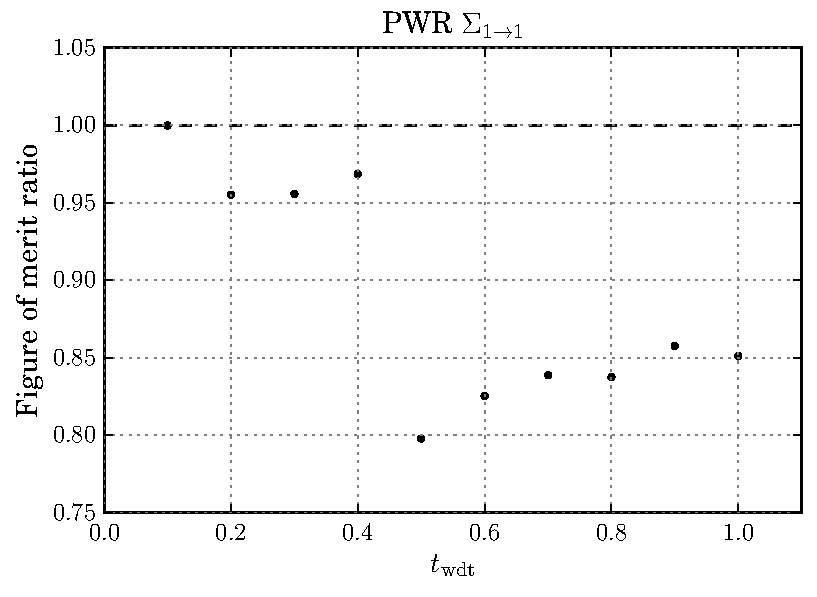
\includegraphics[scale=0.6]{images/results/pwr_inf_sp0_grp_1} &
  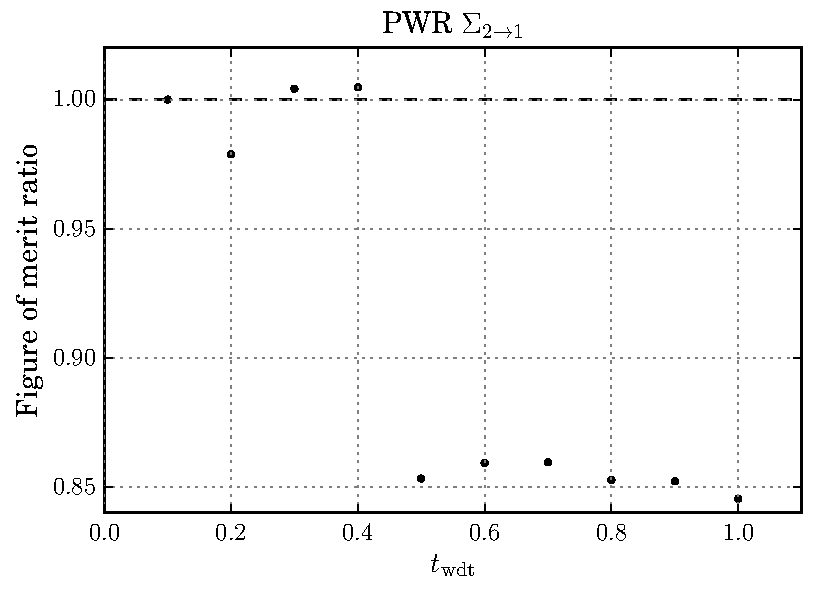
\includegraphics[scale=0.6]{images/results/pwr_inf_sp0_grp_2} \\
    (a) & (b) \\
  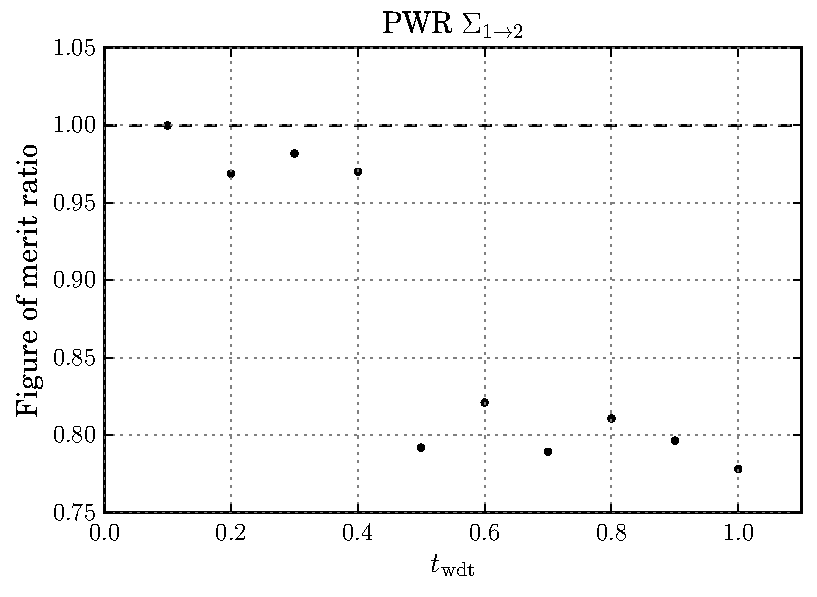
\includegraphics[scale=0.6]{images/results/pwr_inf_sp0_grp_3} &
  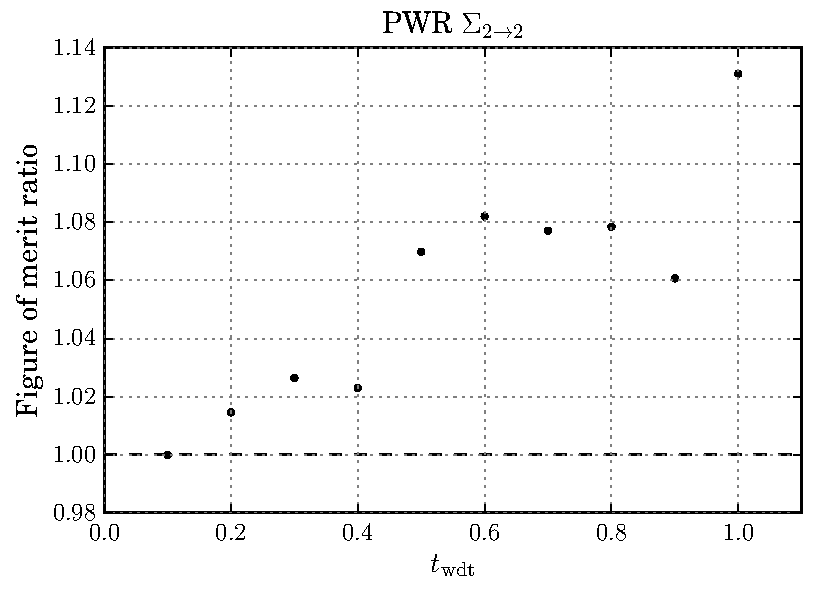
\includegraphics[scale=0.6]{images/results/pwr_inf_sp0_grp_4} \\
    (c) & (d)
  \end{tabular}
  \caption[Figure of merit ratio of the infinite zeroth-moment of the
  scattering cross-section for the PWR]{Figure of merit ratio of the
    infinite zeroth-moment of the scattering cross-section $S_0$ for
    the PWR vs the \gls{wdt} threshold for the (a) $\Sigma_{1 \to
      1}$, (b) $\Sigma_{2 \to 1}$, (c) $\Sigma_{1 \to 2}$ and (d)
    $\Sigma_{2 \to 2}$ entries. The group boundary is at $0.0625$ eV. \gls{fom} is
    calculated using the last 20 data points.}
  \label{fig:pwr_inf_sp0}
\end{figure}
\newpage
\subsection{Discussion}
\label{sec:pwr_discussion}

There is no clear value of the \gls{wdt} threshold that improves
\gls{fom} for all cases. Depending on the desired output parameters of
the simulation, using \gls{wdt} may be beneficial. We observe an
improvement or parity in infinite flux for both groups across all values of
$t_\mathrm{wdt}$. Therefore, we should look to other parameters to
determine a useful value of $t_{\mathrm{wdt}}$.

The infinite total cross-section for the slow group is similarly
improved, but the fast group data show a consistent under performance
as shown in Fig.~\ref{fig:pwr_inf_tot} and
Tab.~\ref{tab:pwr_inf_tot}. Values of $t_{\mathrm{wdt}} \geq 0.5$
result in the largest reduction, these values have a mean \gls{fom}
ratio of 0.81. Lower values $0.1 \leq t_{\mathrm{wdt}} \leq 0.4$ have
a mean \gls{fom} ratio of 0.92.

We see a similar pattern in the entries in the scattering matrix, as
shown in Fig.~\ref{fig:pwr_inf_sp0} and
Tab.~\ref{tab:pwr_inf_sp0}. The slow-group inscattering cross-section
has a consistent improvement, while the fast group underperforms. For
the fast group scattering into either group, as with infinite total
cross-section, there are two domains. When
$0.1 \leq t_{\mathrm{wdt}} \leq 0.4$, the ratio is between 0.95 and
unity, and is much lower otherwise. These data, therefore, suggest the
same range of \gls{wdt} threshold as the infinite total
cross-section. For the upscattering cross-section $\Sigma_{2 \to 1}$,
two values within this range return an improvement in \gls{fom} ratio,
$t_\mathrm{wdt} = 0.3, 0.4$.

Overall the ratio data indicate that a \gls{wdt} threshold of
$t_{\mathrm{wdt}} = 0.3$ or $t_{\mathrm{wdt}} = 0.4$ provides an
improvement in the statistics for thermal neutrons, without much loss
of statistics elsewhere. The final \gls{fom} ratios for these values
are summarized in Tab.~\ref{tab:pwr_results}. If the thermal group
infinite parameters discussed here for a \gls{pwr} are desired with
high accuracy, the \gls{wdt} method provides a means to improve these
statistics without causing a significant impact on the fast group.

\begin{table}[hbtp]
  \centering
  \caption[Summary of \acrshort{fom} ratios for the PWR for select
    cases.]{Summary of \acrshort{fom} ratios for the PWR for select
    cases of \gls{wdt} threshold.}
  \begin{tabular}{cc} $t_{\mathrm{wdt}}=0.3$ &  $t_{\mathrm{wdt}}=0.4$ \\
  \begin{tabular}{lr}\toprule
    \textbf{Parameter}& $\overline{\mathbf{FOM}}$ \textbf{Ratio} \\ \midrule
    $\phi_{1, \infty}$ & 1.017769 \\
    $\phi_{2, \infty}$ & 1.040053 \\
    $\Sigma_{1,t}$ & 0.956974 \\
    $\Sigma_{2,t}$ & 1.020527 \\
    $\Sigma_{1 \to 1}$ & 0.955936 \\
    $\Sigma_{2 \to 1}$ & 1.004215 \\
    $\Sigma_{1 \to 2}$ & 0.981914 \\
    $\Sigma_{2 \to 2}$ & 1.004215 \\ \bottomrule
  \end{tabular}&
  \begin{tabular}{lr}\toprule
    \textbf{Parameter}& $\overline{\mathbf{FOM}}$ \textbf{Ratio} \\ \midrule
    $\phi_{1, \infty}$ & 1.050233 \\
    $\phi_{2, \infty}$ & 1.019965 \\
    $\Sigma_{1,t}$ & 0.967552 \\
    $\Sigma_{2,t}$ & 1.013200 \\
    $\Sigma_{1 \to 1}$ & 0.968628 \\
    $\Sigma_{2 \to 1}$ & 1.004753 \\
    $\Sigma_{1 \to 2}$ & 0.970194 \\
    $\Sigma_{2 \to 2}$ & 1.004753 \\ \bottomrule
  \end{tabular}
  \end{tabular}
  \label{tab:pwr_results}
\end{table}

\newpage
\section{Fast reactor pin cell}
\label{sec:fast_pin_cell}

We adapted the fast reactor pin cell from another example provided in
the Serpent validation files~\cite{serpent_web}. This is a lead cooled
pin cell with \gls{mox} fuel containing Uranium, Plutonium and a small
amount of Americium. The cladding is stainless steel. The lattice is
hexagonal, and has reflective boundary conditions. As with the
\gls{pwr} pin cell, we ran the simulation with two energy
groups with the group boundary at 0.625 eV.

\begin{figure}[hbtp]
  \centering
  \begin{tabular}{cc}
  
\includegraphics[scale=0.5]{images/results/fast_pin_geom1} \\
\begin{tabular}{@{}lr@{}}
\toprule
\textbf{Parameter}     & \textbf{Value (cm)} \\ \midrule
Void radius     & 0.1          \\
Pellet radius & 0.45          \\
Inner cladding radius & 0.465          \\
Outer cladding radius & 0.525          \\
Pitch              & 1.789          \\ \bottomrule
\end{tabular}
  \end{tabular}
  \caption[Fast pin cell geometry and physical parameters.]{Fast pin
    cell geometry and physical parameters. The pellet is shown in
    blue, the cladding green, and the coolant orange. Black regions
    are voids.}
  \label{fig:fast}
\end{figure}

\subsection{Infinite flux}
\label{sec:fast_inf_flx}
A summary of the \gls{fom} ratio,
$\overline{\mathrm{FOM}}(t_{\mathrm{wdt}})$, for the fast reactor pin
cell for infinite flux ($\phi_{\infty}$) is shown in Tab.~\ref{tab:fast_inf_flx} and
shown graphically in Fig.~\ref{fig:fast_inf_flx}. The \gls{fom} ratio
group 1 is consistently higher; for group 2 the \gls{fom} values are
very low, so the ratios are not as useful. Although there appears to
be a high ratio (3.140) at the threshold value $t_{\mathrm{wdt}}
=0.4$, this merely reflects the poor statistics. As seen in
Fig.~\ref{fig:fast_inf_flx_example}, the \gls{fom} is not converging
to a single value as shown earlier.
\begin{table}[hbtp]
  \centering
  \caption[$\overline{\mathrm{FOM}}$ and ratio for
    the fast pin cell infinite flux.]{$\overline{\mathrm{FOM}}$ as a function of
    $t_{\mathrm{wdt}}$ and the ratio of values to the base case for
    the fast pin cell infinite flux.}
  \begin{tabular}{cc} Group 1 ($E > 0.0625$) & Group 2 \\
    \begin{tabular}{lrr}
\toprule
$t_{\mathrm{wdt}}$ & $\overline{\mathrm{FOM}}$ &    Ratio \\
\midrule
               0.1 &   1.398529$\times 10^{6}$ & 1.000000 \\
               0.2 &   1.458968$\times 10^{6}$ & 1.043217 \\
               0.3 &   1.639208$\times 10^{6}$ & 1.172095 \\
               0.4 &   1.715773$\times 10^{6}$ & 1.226841 \\
               0.5 &   1.688965$\times 10^{6}$ & 1.207673 \\
               0.6 &   1.903000$\times 10^{6}$ & 1.360716 \\
               0.7 &   1.858063$\times 10^{6}$ & 1.328584 \\
               0.8 &   1.818223$\times 10^{6}$ & 1.300097 \\
               0.9 &   1.758294$\times 10^{6}$ & 1.257245 \\
               1.0 &   1.581456$\times 10^{6}$ & 1.130800 \\
\bottomrule
\end{tabular}

 &
   \begin{tabular}{lrr}
\toprule
$t_{\mathrm{wdt}}$ & $\overline{\mathrm{FOM}}$ &    Ratio \\
\midrule
               0.1 &  5.027779$\times 10^{-4}$ & 1.000000 \\
               0.2 &  4.567251$\times 10^{-4}$ & 0.908403 \\
               0.3 &  2.867434$\times 10^{-4}$ & 0.570318 \\
               0.4 &  1.578718$\times 10^{-3}$ & 3.139990 \\
               0.5 &  4.364983$\times 10^{-4}$ & 0.868173 \\
               0.6 &  3.411268$\times 10^{-4}$ & 0.678484 \\
               0.7 &  3.863250$\times 10^{-4}$ & 0.768381 \\
               0.8 &  4.222281$\times 10^{-4}$ & 0.839790 \\
               0.9 &   0.000000$\times 10^{0}$ & 0.000000 \\
               1.0 &  2.816380$\times 10^{-4}$ & 0.560164 \\
\bottomrule
\end{tabular}

  \end{tabular}
\label{tab:fast_inf_flx}
\end{table}
\begin{figure}[hbtp]
  \centering
  \begin{tabular}{c}
  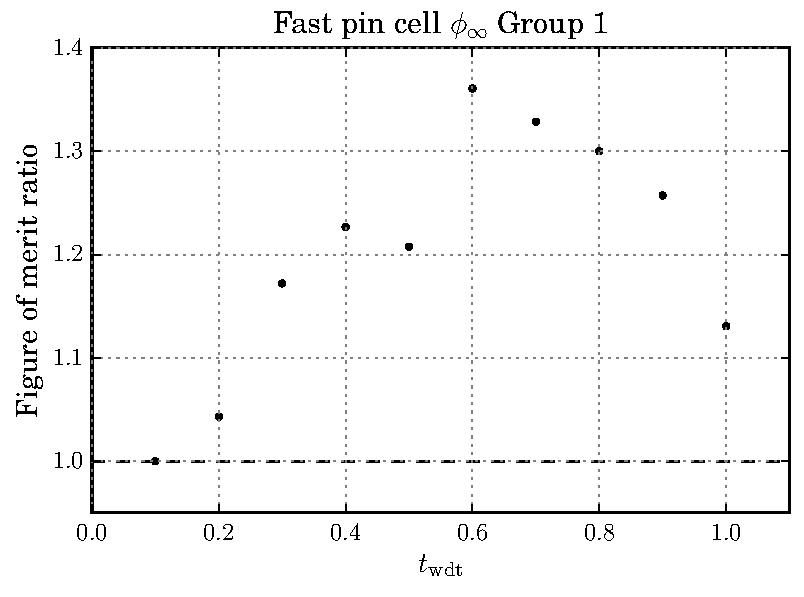
\includegraphics[scale=0.9]{images/results/fast_inf_flx_grp_1} \\
    (a) \\
  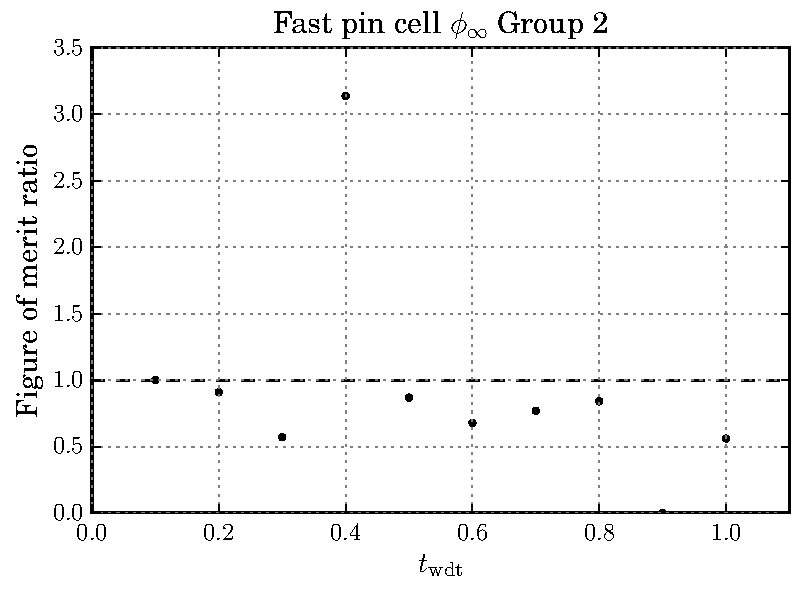
\includegraphics[scale=0.9]{images/results/fast_inf_flx_grp_2} \\
    (b) 
  \end{tabular}
  \caption[Figure of merit ratio of the infinite flux for the
  PWR]{Figure of merit ratio of the infinite flux for the fast pin cell vs the
    \gls{wdt} threshold for the (a) high and (b) low energy
    groups. The group boundary is at $0.0625$ eV. \gls{fom} is
    calculated using the last 20 data points.}
  \label{fig:fast_inf_flx}
\end{figure}
\begin{figure}[hbtp]
  \centering
  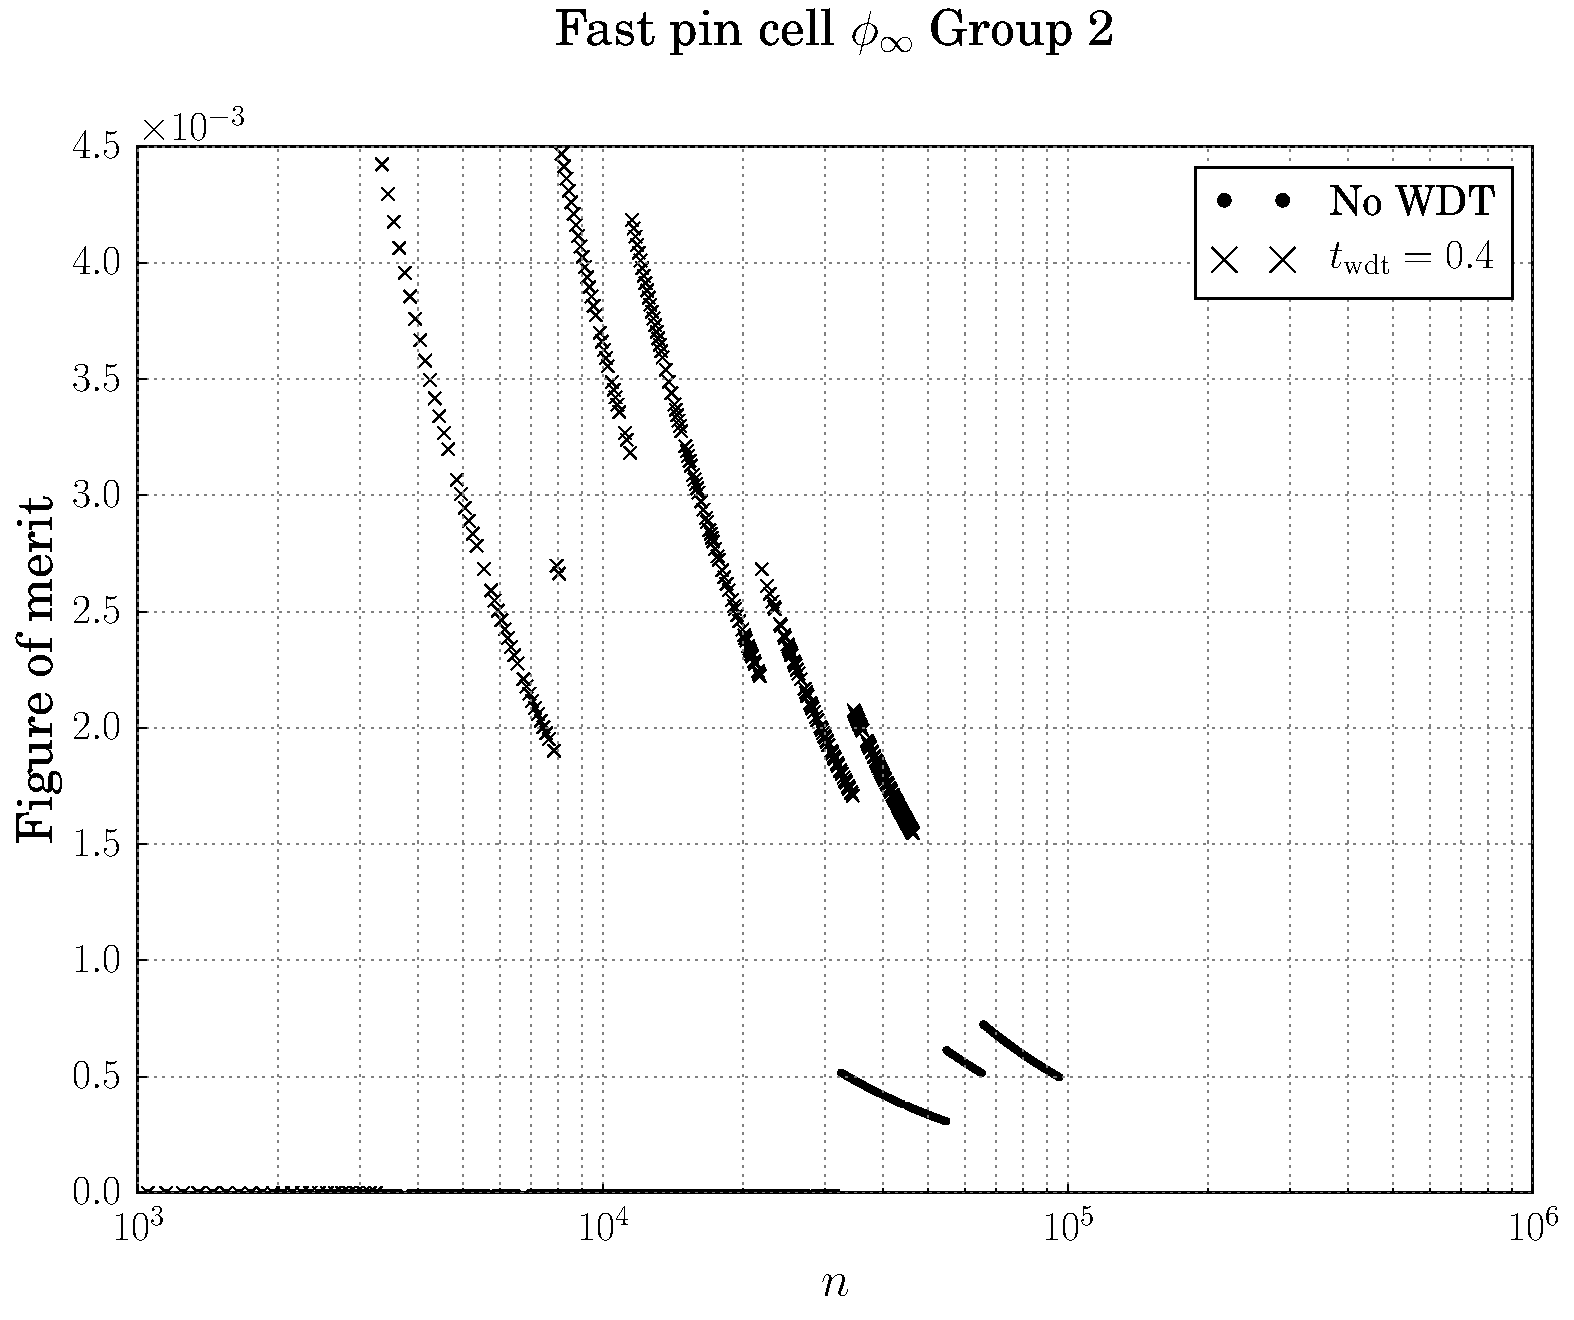
\includegraphics[scale=0.5]{images/results/fast_inf_flx_example}
  \caption[\Acrshort{fom} convergence for $\phi_{\infty}$ for the base
  and $t_{\mathrm{wdt}} = 0.4$ case for group 2.]{\Acrshort{fom} convergence for
    $\phi_{\infty}$ the base and $t_{\mathrm{wdt}} = 0.4$ case for
    group 2.}
  \label{fig:fast_inf_flx_example}
\end{figure}

\subsection{Infinite total cross-section}
\label{sec:fast_inf_tot_cross_section}
A summary of the \gls{fom} ratio,
$\overline{\mathrm{FOM}}(t_{\mathrm{wdt}})$, for the fast reactor pin
cell for infinite total cross-section ($\Sigma_{t,
  \infty}$) is shown in Tab.~\ref{tab:fast_inf_tot} and shown
graphically in Fig.~\ref{fig:fast_inf_tot}. The \gls{fom} ratio for
group 1 is higher for all values of $t_{\mathrm{wdt}}$ with the
exception of 0.2. For group 2, as seen in Sec.~\ref{sec:fast_inf_flx}, the
\gls{fom} values are very low, and one ratio is artificially inflated
when $t_{\mathrm{wdt}} = 0.6$
due to the lack of convergence. This case is shown in
Fig.~\ref{fig:fast_inf_tot_example}; there are not enough statistics
for the low energy group to cause the \gls{fom} to converge to a high
enough value to be significant.
\begin{table}[hbtp]
  \centering
  \caption[$\overline{\mathrm{FOM}}$ and ratio for
    the fast reactor pin cell $\Sigma_{t,\infty}$.]{$\overline{\mathrm{FOM}}$ as a function of
    $t_{\mathrm{wdt}}$ and the ratio of values to the base case for
    the fast reactor pin cell $\Sigma_{t,\infty}$.}
  \begin{tabular}{cc} Group 1 ($E > 0.0625$) & Group 2 \\
    \begin{tabular}{lrr}
\toprule
$t_{\mathrm{wdt}}$ & $\overline{\mathrm{FOM}}$ &    Ratio \\
\midrule
               0.1 &   1.136275$\times 10^{7}$ & 1.000000 \\
               0.2 &   1.126136$\times 10^{7}$ & 0.991077 \\
               0.3 &   1.248018$\times 10^{7}$ & 1.098342 \\
               0.4 &   1.306365$\times 10^{7}$ & 1.149691 \\
               0.5 &   1.278691$\times 10^{7}$ & 1.125336 \\
               0.6 &   1.382315$\times 10^{7}$ & 1.216532 \\
               0.7 &   1.239126$\times 10^{7}$ & 1.090516 \\
               0.8 &   1.343677$\times 10^{7}$ & 1.182529 \\
               0.9 &   1.325812$\times 10^{7}$ & 1.166806 \\
               1.0 &   1.192159$\times 10^{7}$ & 1.049182 \\
\bottomrule
\end{tabular}

 &
   \begin{tabular}{lrr}
\toprule
$t_{\mathrm{wdt}}$ & $\overline{\mathrm{FOM}}$ &     Ratio \\
\midrule
               0.1 &  8.481607$\times 10^{-3}$ &  1.000000 \\
               0.2 &  9.381356$\times 10^{-4}$ &  0.110608 \\
               0.3 &  5.493018$\times 10^{-4}$ &  0.064764 \\
               0.4 &  3.177720$\times 10^{-3}$ &  0.374660 \\
               0.5 &  6.372709$\times 10^{-4}$ &  0.075136 \\
               0.6 &  3.224228$\times 10^{-1}$ & 38.014350 \\
               0.7 &  4.215556$\times 10^{-4}$ &  0.049702 \\
               0.8 &  7.736467$\times 10^{-4}$ &  0.091215 \\
               0.9 &   0.000000$\times 10^{0}$ &  0.000000 \\
               1.0 &  9.794372$\times 10^{-4}$ &  0.115478 \\
\bottomrule
\end{tabular}

  \end{tabular}
\label{tab:fast_inf_tot}
\end{table}
\begin{figure}[hbtp]
  \centering
  \begin{tabular}{c}
  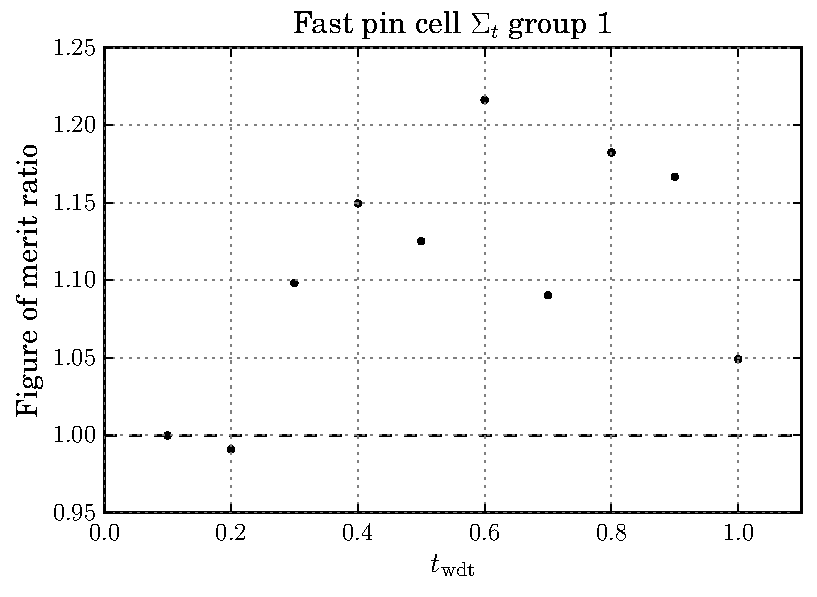
\includegraphics[scale=0.9]{images/results/fast_inf_tot_grp_1} \\
    (a) \\
  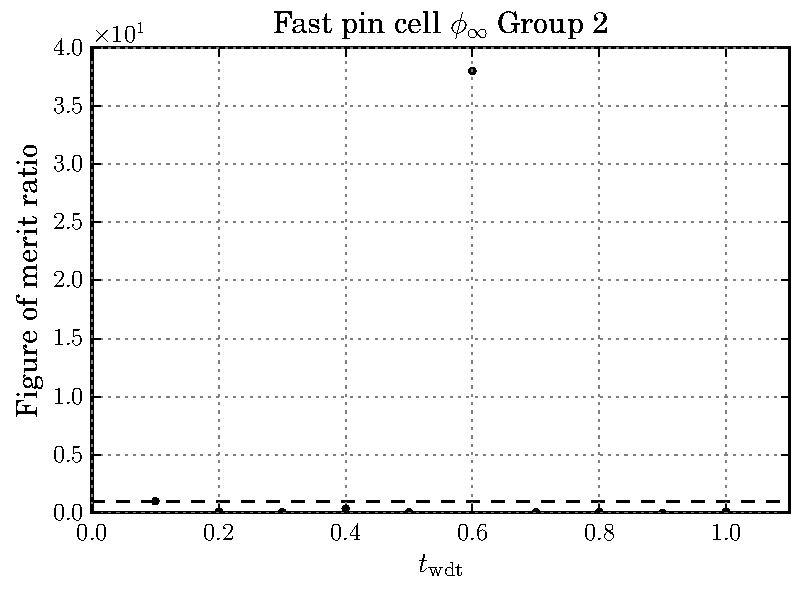
\includegraphics[scale=0.9]{images/results/fast_inf_tot_grp_2} \\
    (b) 
  \end{tabular}
  \caption[Figure of merit ratio of the $\Sigma_{t,\infty}$ for the
  fast reactor pin cell]{Figure of merit ratio of
    $\Sigma_{t,\infty}$ for the fast reactor pin cell vs the \gls{wdt}
    threshold for (a) group 1 and (b) group 2. The group
    boundary is at $0.0625$ eV. \gls{fom} is calculated using the last
    20 data points.}
  \label{fig:fast_inf_tot}
\end{figure}
\begin{figure}[hbtp]
  \centering
  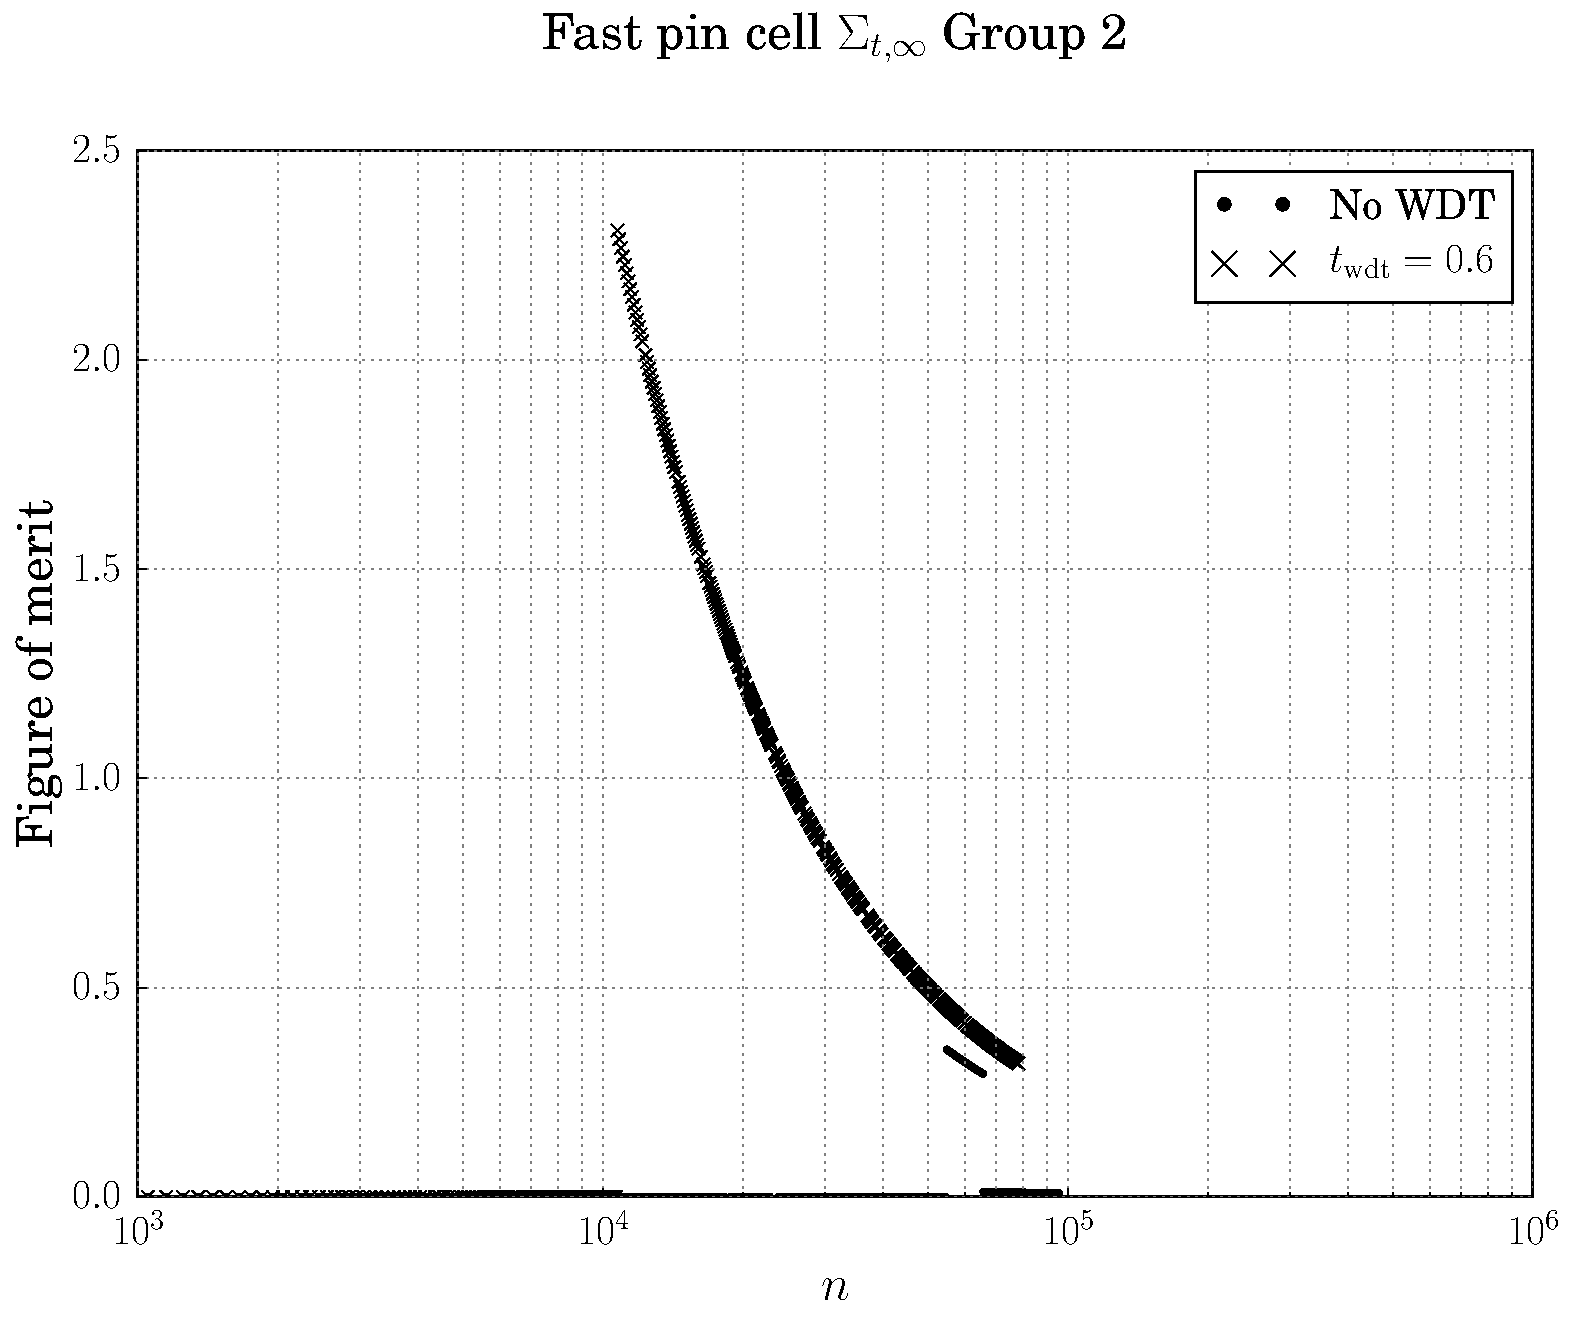
\includegraphics[scale=0.5]{images/results/fast_inf_tot_example}
  \caption[\Acrshort{fom} convergence for $\Sigma_{t,\infty}$ the base
  and $t_{\mathrm{wdt}} = 0.6$ case.]{\Acrshort{fom} convergence for
    $\Sigma_{t,\infty}$ the base and $t_{\mathrm{wdt}} = 0.6$ case.}
  \label{fig:fast_inf_tot_example}
\end{figure}

\subsection{Scattering Matrices}
\label{sec:fast_inf_sp0}

For the two-group case, the scattering matrices for the zeroth
moments $S_0$ is $2 \times 2$. A summary of the \gls{fom} ratio
for the zeroth moment $S_0$ is shown in Table~\ref{tab:fast_inf_sp0}. The
tables are for the entry in row $g$ and column $g'$, which represents
scattering from group $g'$ into group $g$, indicated as $g' \to g$.

The group 1 inscattering matrix displays good statistics, the other
three entries have an extremely low \gls{fom}, indicating that there
are not enough statistics. The group 1 inscattering \gls{fom} ratio is
plotted in Fig.~\ref{fig:fast_inf_sp0}. \gls{wdt} returns a higher
\gls{fom} for all values of $t_{\mathrm{wdt}} \geq 0.3$, and close to
parity for $t_{\mathrm{wdt}} = 0.2$.

\begin{table}[hbtp]
  \centering
  \caption[$\overline{\mathrm{FOM}}$ and ratio for
  the fast reactor pin cell infinite $S_0$ scattering matrix.]{$\overline{\mathrm{FOM}}$ as a function of
    $t_{\mathrm{wdt}}$ and the ratio of values to the base case for
    the fast reactor pin cell infinite $S_0$ scattering matrix}
  \begin{tabular}{cc} $\Sigma_{1\to 1}$ & $\Sigma_{2 \to 1}$ \\
\begin{tabular}{lrr}
\toprule
$t_{\mathrm{wdt}}$ & $\overline{\mathrm{FOM}}$ &    Ratio \\
\midrule
               0.1 &   1.025750$\times 10^{7}$ & 1.000000 \\
               0.2 &   1.026018$\times 10^{7}$ & 1.000262 \\
               0.3 &   1.140244$\times 10^{7}$ & 1.111619 \\
               0.4 &   1.203271$\times 10^{7}$ & 1.173064 \\
               0.5 &   1.224380$\times 10^{7}$ & 1.193644 \\
               0.6 &   1.375806$\times 10^{7}$ & 1.341268 \\
               0.7 &   1.246229$\times 10^{7}$ & 1.214944 \\
               0.8 &   1.356487$\times 10^{7}$ & 1.322435 \\
               0.9 &   1.334051$\times 10^{7}$ & 1.300561 \\
               1.0 &   1.221318$\times 10^{7}$ & 1.190659 \\
\bottomrule
\end{tabular}
 & 
\begin{tabular}{lrr}
\toprule
$t_{\mathrm{wdt}}$ & $\overline{\mathrm{FOM}}$ &    Ratio \\
\midrule
               0.1 &   0.000000$\times 10^{0}$ & 0.000000 \\
               0.2 &  3.461351$\times 10^{-4}$ & 0.000346 \\
               0.3 &  2.464090$\times 10^{-4}$ & 0.000246 \\
               0.4 &  1.541451$\times 10^{-3}$ & 0.001541 \\
               0.5 &  3.324048$\times 10^{-4}$ & 0.000332 \\
               0.6 &   0.000000$\times 10^{0}$ & 0.000000 \\
               0.7 &  7.124125$\times 10^{-4}$ & 0.000712 \\
               0.8 &  3.543062$\times 10^{-4}$ & 0.000354 \\
               0.9 &   0.000000$\times 10^{0}$ & 0.000000 \\
               1.0 &  6.957632$\times 10^{-4}$ & 0.000696 \\
\bottomrule
\end{tabular}
 \\
$\Sigma_{1\to 2}$ & $\Sigma_{2 \to 2}$ \\
\begin{tabular}{lrr}
\toprule
$t_{\mathrm{wdt}}$ & $\overline{\mathrm{FOM}}$ &    Ratio \\
\midrule
               0.1 &   0.000000$\times 10^{0}$ & 0.000000 \\
               0.2 &   0.000000$\times 10^{0}$ & 0.000000 \\
               0.3 &   0.000000$\times 10^{0}$ & 0.000000 \\
               0.4 &   0.000000$\times 10^{0}$ & 0.000000 \\
               0.5 &   0.000000$\times 10^{0}$ & 0.000000 \\
               0.6 &   0.000000$\times 10^{0}$ & 0.000000 \\
               0.7 &   0.000000$\times 10^{0}$ & 0.000000 \\
               0.8 &   0.000000$\times 10^{0}$ & 0.000000 \\
               0.9 &   0.000000$\times 10^{0}$ & 0.000000 \\
               1.0 &   0.000000$\times 10^{0}$ & 0.000000 \\
\bottomrule
\end{tabular}
 & 
\begin{tabular}{lrr}
\toprule
$t_{\mathrm{wdt}}$ & $\overline{\mathrm{FOM}}$ &    Ratio \\
\midrule
               0.1 &   0.000000$\times 10^{0}$ & 0.000000 \\
               0.2 &  6.991410$\times 10^{-4}$ & 0.000699 \\
               0.3 &  2.464090$\times 10^{-4}$ & 0.000246 \\
               0.4 &  3.295802$\times 10^{-4}$ & 0.000330 \\
               0.5 &   0.000000$\times 10^{0}$ & 0.000000 \\
               0.6 &   0.000000$\times 10^{0}$ & 0.000000 \\
               0.7 &   0.000000$\times 10^{0}$ & 0.000000 \\
               0.8 &  3.543062$\times 10^{-4}$ & 0.000354 \\
               0.9 &   0.000000$\times 10^{0}$ & 0.000000 \\
               1.0 &  2.317413$\times 10^{-4}$ & 0.000232 \\
\bottomrule
\end{tabular}
 
  \end{tabular}
  \label{tab:fast_inf_sp0}
\end{table}
\begin{figure}[hbtp]
  \centering
  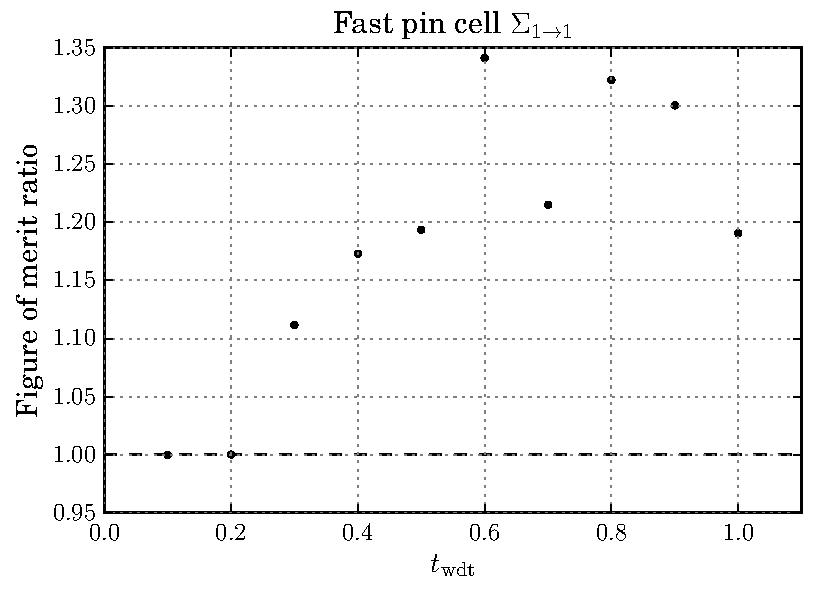
\includegraphics[scale=0.9]{images/results/fast_inf_sp0_grp_1}
  \caption[Figure of merit ratio $\Sigma_{1 \to 1}$ for the fast reactor pin cell]{Figure of
    merit ratio of $\Sigma_{1 \to 1}$ for
    the fast reactor pin cell. The group boundary is at $0.0625$ eV. \gls{fom} is calculated
    using the last 20 data points.}
  \label{fig:fast_inf_sp0}
\end{figure}

\newpage

\subsection{Discussion}
\label{sec:fast_discussion}

There is very little thermal flux in a fast reactor. This results in
poor statistics for that group, a fact that \gls{wdt} does not
remedy. As evidenced by the results presenting in this section, all
values of $t_{\mathrm{wdt}}$ continued to result in group 2 \gls{fom} orders
of magnitude smaller than both group 1 for this problem, and either
group for the \gls{pwr}.

For the fast group, there is consistent improvement in the \gls{fom}
for all values of $t_{\mathrm{wdt}}$. The \gls{fom} ratio peaks at
$t_{\mathrm{wdt}} = 0.6$ for the infinite flux, total cross-section
and group 1 inscattering cross-section. This value represents the
highest improvement in group 1, and the values are summarized in
Tab.~\ref{tab:fast_discussion}. The values for group 2 are omitted as
this value, like all others, did not result in meaningful improvement.

\begin{table}[hbtp]
  \centering
  \caption{Summary of \acrshort{fom} ratios for the fast reactor pin
  cell for $t_{\mathrm{wdt}}$ = 0.6.}
  \begin{tabular}{lr}\toprule
    \textbf{Parameter}& $\overline{\mathbf{FOM}}$ \textbf{Ratio} \\ \midrule
    $\phi_{1, \infty}$ & 1.360716 \\
    $\Sigma_{1,t}$ & 1.216532 \\
    $\Sigma_{1 \to 1}$ & 1.341268 \\ \bottomrule
  \end{tabular}
  \label{tab:fast_discussion}
\end{table}


\newpage
\section{Homogenous fuel element}
\label{sec:homog}

The third test case is derived from the \gls{treat} reactor at
\gls{inl}. Work at \gls{inl} focuses on using deterministic solvers to
model the core, the Serpent 2 Monte Carlo code is used to generate the
cross-sections for these solvers. We used a homogenized fuel element
that replicates the material but not geometry of the \gls{treat}
fuel. The simulation uses eleven energy groups, which replicates the
groups used by the deterministic solvers. This group structure is
summarized in Table.~\ref{tab:homog_energy}.
\begin{table}[hbtp]
  \centering
  \caption{Energy group structure for the homogenous fuel element.}
  \begin{tabular}{cc}
  \begin{tabular}{rr} \toprule
    \textbf{Group}& \textbf{Upper energy limit (MeV)} \\ \midrule
    1 & 20.0000  \\
    2 & 3.32870  \\
    3 & 1.15620 $\times 10^{-1}$ \\
    4 & 3.48110 $\times 10^{-3}$ \\
    5 & 1.32700 $\times 10^{-4}$ \\
    6 & 8.10003 $\times 10^{-6}$ \\ \bottomrule
  \end{tabular} &
  \begin{tabular}{rr} \toprule
    \textbf{Group}& \textbf{Upper energy limit (MeV)} \\ \midrule
    7 & 6.25000 $\times 10^{-7}$ \\
    8 & 2.09610 $\times 10^{-7}$ \\
    9 & 7.64970 $\times 10^{-8}$ \\
    10 & 4.73020 $\times 10^{-8}$ \\
    11 & 2.00100 $\times 10^{-8}$ \\ \\\bottomrule
  \end{tabular}
  \end{tabular}
  \label{tab:homog_energy}
\end{table}
To simplify the analysis, and to allow comparison between the other
two test cases, these groups can be collapsed. The values we are
considering, $\phi_{\infty}$, $\Sigma_{t,\infty}$, and the zeroth
scattering matrix are all independent measurements with regard to
energy. We can sum all the $\phi_{\infty}$ for each energy group to
get a total $\phi_{\infty}$ for the entire energy range. As there is
no covariance, the variance of the sum will be the sum of the
variance~\cite{taylor1997}. The variance for summing energy groups $g$ to $g'$ is therefore:
\begin{equation*}
  \mathrm{Var}\left( \sum_{j=g}^{g'}\phi_{g,\infty}\right) =   \sum_{j=g}^{g'}\mathrm{Var}\left(\phi_{g,\infty}\right)
\end{equation*}
This allows us to collapse groups one through six into a single group,
hereafter denoted by an $f$ for fast and groups seven through eleven as
 a slow group, $s$. The boundary of group seven aligns with the separation
of the two groups in the previous test problems, so we can compare the
results in a more natural
fashion. Fig.~\ref{fig:homog_fom_convergence_example} shows the
\gls{fom} convergence for the combined fast group. As expected, the
combined group shows the same convergence characteristic as the single
groups.

\begin{figure}[hbtp]
  \centering
  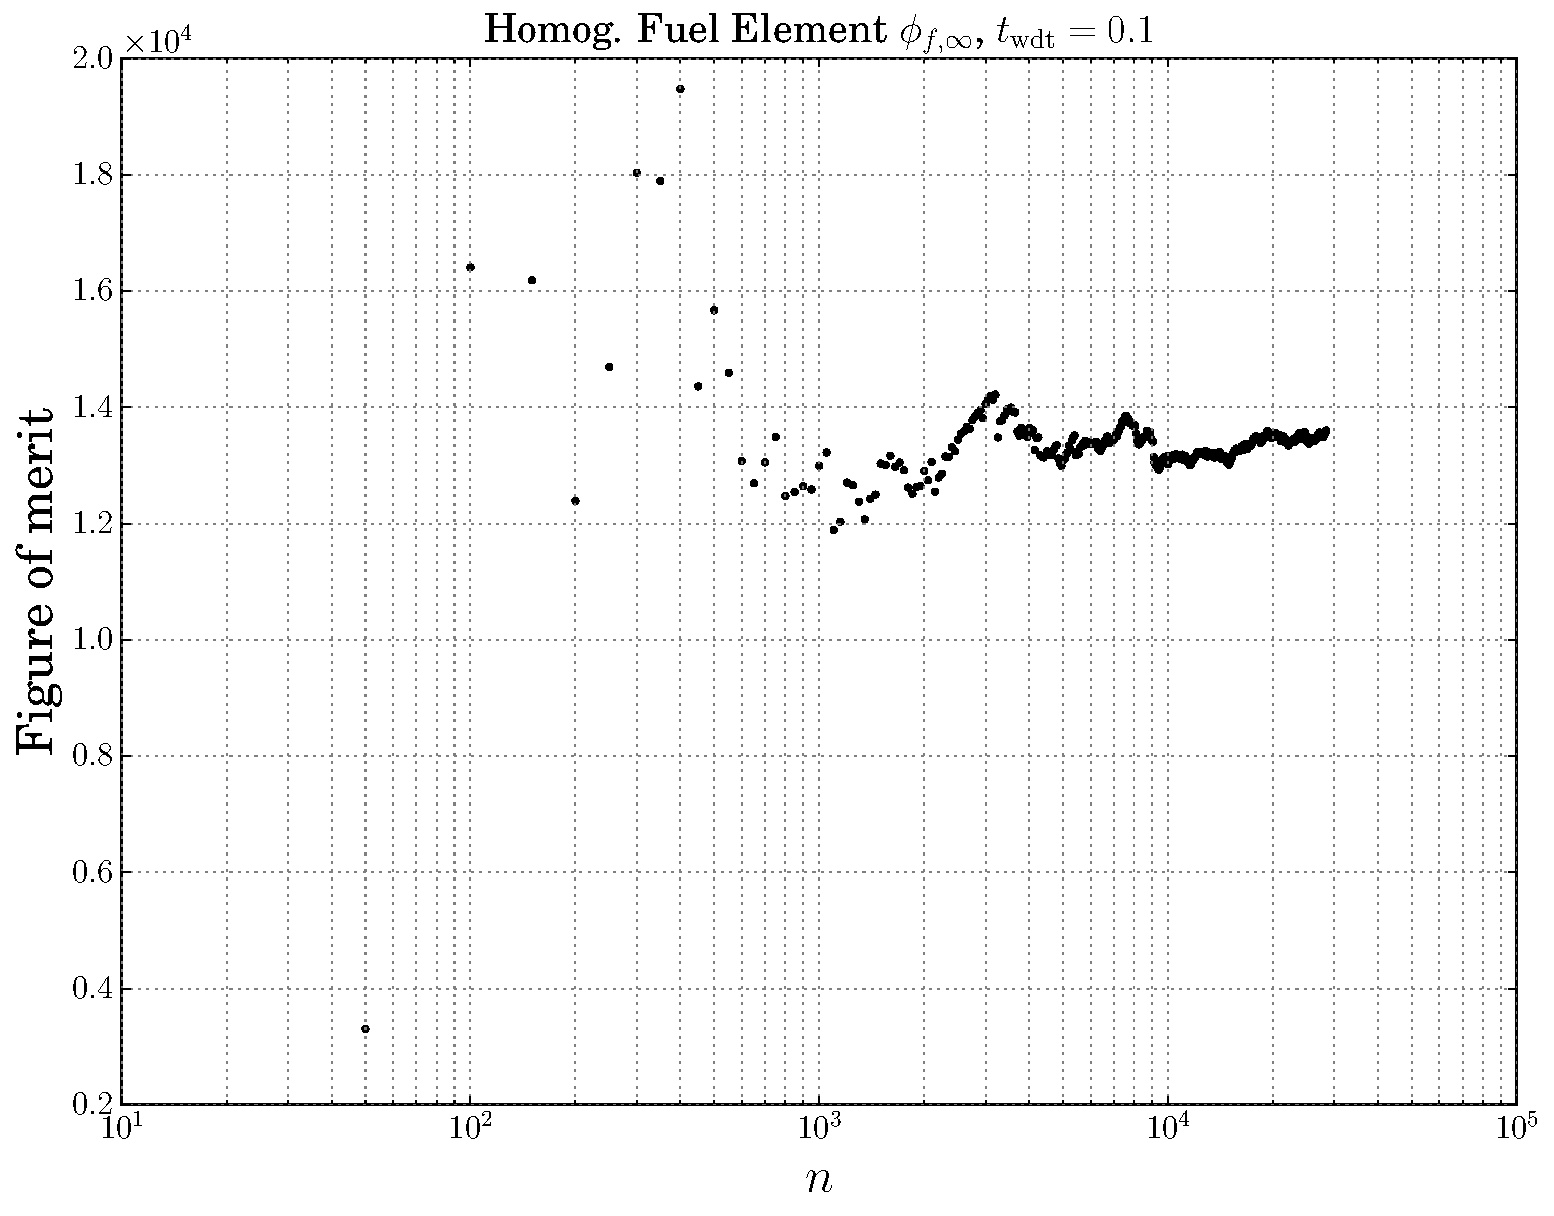
\includegraphics[scale=0.5]{images/homog_fom_convergence_example}
  \caption{Convergence of $\phi_{\infty}$ for the combined fast group
    for the homogenous fuel element for the base case
    $t_{\mathrm{wdt}} = 0.1$.}
  \label{fig:homog_fom_convergence_example}
\end{figure}

\subsection{Infinite flux}
\label{sec:homog_inf_flx}

A summary of the \gls{fom} ratio,
$\overline{\mathrm{FOM}}(t_{\mathrm{wdt}})$, for the homogenous fuel
element for infinite flux ($\phi_{\infty}$) is shown in
Tab.~\ref{tab:homog_inf_flx} and shown graphically in
Fig.~\ref{fig:homog_inf_flx}. The Tables for all eleven of the
original energy groups are included in
App.~\ref{sec:homog_inf_flx_data}.

As shown in both the table and graphically, we observe an improvement
in \gls{fom} for \gls{wdt} threshold values
$0.2 \leq t_{\mathrm{wdt}} \leq 0.6$ and $t_{\mathrm{wdt}} = 0.8, 1.0$ for
the fast group. The improvement is moderate for this
group, with a maximum improvement of 1.07 times the base case. The
improvements are even slighter for the slow group, where we observe a
maximum of 1.014 times the base case for $0.4 \leq t_{\mathrm{wdt}} 0.6$ and $t_{\mathrm{wdt}} = 1.0$.

\begin{table}[hbtp]
  \centering
  \caption[$\overline{\mathrm{FOM}}$ and ratio for
    the homogenous fuel element infinite flux.]{$\overline{\mathrm{FOM}}$ as a function of
    $t_{\mathrm{wdt}}$ and the ratio of values to the base case for
    the homogenous fuel element infinite flux.}
  \begin{tabular}{cc} Fast Group ($E > 0.0625$) & Slow Group \\
    \begin{tabular}{lrr}
\toprule
$t_{\mathrm{wdt}}$ & $\overline{\mathrm{FOM}}$ &    Ratio \\
\midrule
               0.1 &   1.354229$\times 10^{4}$ & 1.000000 \\
               0.2 &   1.373594$\times 10^{4}$ & 1.014299 \\
               0.3 &   1.409053$\times 10^{4}$ & 1.040483 \\
               0.4 &   1.444534$\times 10^{4}$ & 1.066684 \\
               0.5 &   1.398881$\times 10^{4}$ & 1.032972 \\
               0.6 &   1.372165$\times 10^{4}$ & 1.013244 \\
               0.7 &   1.341316$\times 10^{4}$ & 0.990465 \\
               0.8 &   1.359856$\times 10^{4}$ & 1.004155 \\
               0.9 &   1.347952$\times 10^{4}$ & 0.995365 \\
               1.0 &   1.433894$\times 10^{4}$ & 1.058826 \\
\bottomrule
\end{tabular}

 &
   \begin{tabular}{lrr}
\toprule
$t_{\mathrm{wdt}}$ & $\overline{\mathrm{FOM}}$ &    Ratio \\
\midrule
               0.1 &   3.309991$\times 10^{4}$ & 1.000000 \\
               0.2 &   3.189448$\times 10^{4}$ & 0.963582 \\
               0.3 &   3.189179$\times 10^{4}$ & 0.963501 \\
               0.4 &   3.338953$\times 10^{4}$ & 1.008750 \\
               0.5 &   3.355018$\times 10^{4}$ & 1.013604 \\
               0.6 &   3.338649$\times 10^{4}$ & 1.008658 \\
               0.7 &   3.271800$\times 10^{4}$ & 0.988462 \\
               0.8 &   3.202989$\times 10^{4}$ & 0.967673 \\
               0.9 &   3.283915$\times 10^{4}$ & 0.992122 \\
               1.0 &   3.332469$\times 10^{4}$ & 1.006791 \\
\bottomrule
\end{tabular}

  \end{tabular}
\label{tab:homog_inf_flx}
\end{table}
\begin{figure}[hbtp]
  \centering
  \begin{tabular}{c}
  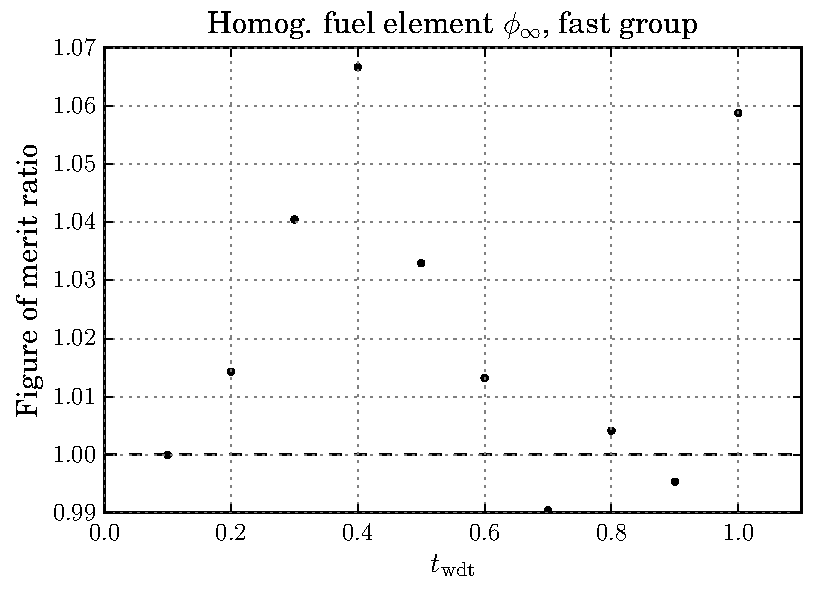
\includegraphics[scale=0.9]{images/results/homog_inf_flx_grp_comb1} \\
    (a) \\
  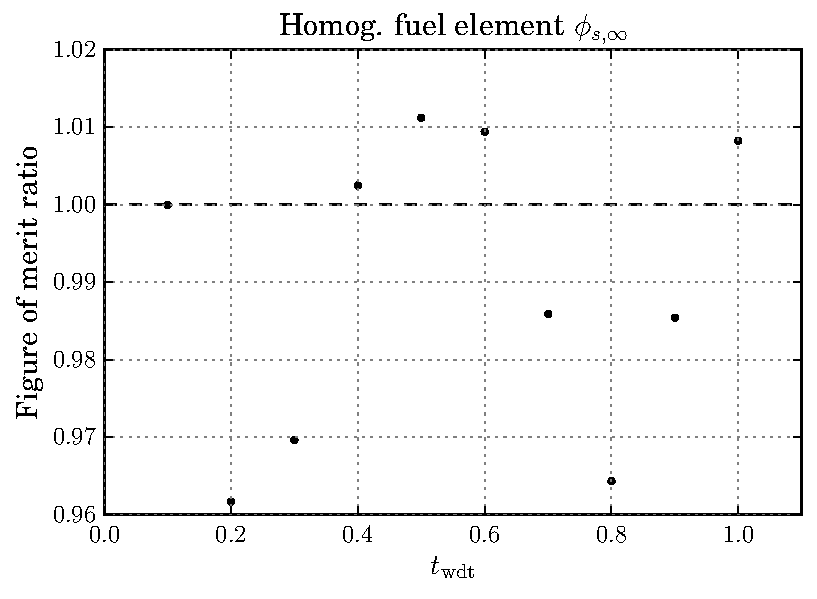
\includegraphics[scale=0.9]{images/results/homog_inf_flx_grp_comb2} \\
    (b) 
  \end{tabular}
  \caption[Figure of merit ratio of the infinite flux for the
  homogeneous fuel element]{Figure of merit ratio of the infinite flux
    for the homogeneous fuel element vs the
    \gls{wdt} threshold for the (a) fast and (b) slow 
    groups. The group boundary is at $0.0625$ eV. \gls{fom} is
    calculated using the last 20 data points.}
  \label{fig:homog_inf_flx}
\end{figure}

\subsection{Infinite total cross-section}
\label{sec:homog_inf_total}

A summary of the \gls{fom} ratio,
$\overline{\mathrm{FOM}}(t_{\mathrm{wdt}})$, for the homogeneous fuel element
 infinite total cross-section is shown in Tab.~\ref{tab:homog_inf_tot} and shown
graphically in Fig.~\ref{fig:homog_inf_tot}. The full data for all
eleven groups is included in App.~\ref{sec:homog_inf_tot_data}.

For both groups, the \gls{wdt} method underperforms the base case in
all but a few select cases. Where it performs better, we observe a very
moderate improvement in \gls{fom}, with the only shared improvement in
both groups at $t_{\mathrm{wdt}} = 0.7$.

\begin{table}[hbtp]
  \centering
  \caption[$\overline{\mathrm{FOM}}$ and ratio for
    the homogeneous fuel element $\Sigma_{t,\infty}$.]{$\overline{\mathrm{FOM}}$ as a function of
    $t_{\mathrm{wdt}}$ and the ratio of values to the base case for
    the homogeneous fuel element $\Sigma_{t,\infty}$.}
  \begin{tabular}{cc} Fast group ($E > 0.0625$) & Slow group \\
    \begin{tabular}{lrr}
\toprule
$t_{\mathrm{wdt}}$ & $\overline{\mathrm{FOM}}$ &    Ratio \\
\midrule
               0.1 &   4.126523$\times 10^{5}$ & 1.000000 \\
               0.2 &   4.165034$\times 10^{5}$ & 1.009333 \\
               0.3 &   3.809894$\times 10^{5}$ & 0.923270 \\
               0.4 &   4.130063$\times 10^{5}$ & 1.000858 \\
               0.5 &   4.317179$\times 10^{5}$ & 1.046202 \\
               0.6 &   3.962803$\times 10^{5}$ & 0.960325 \\
               0.7 &   4.168695$\times 10^{5}$ & 1.010220 \\
               0.8 &   3.989894$\times 10^{5}$ & 0.966890 \\
               0.9 &   4.092305$\times 10^{5}$ & 0.991708 \\
               1.0 &   3.943059$\times 10^{5}$ & 0.955540 \\
\bottomrule
\end{tabular}

 &
   \begin{tabular}{lrr}
\toprule
$t_{\mathrm{wdt}}$ & $\overline{\mathrm{FOM}}$ &    Ratio \\
\midrule
               0.1 &   2.319708$\times 10^{6}$ & 1.000000 \\
               0.2 &   2.242986$\times 10^{6}$ & 0.966926 \\
               0.3 &   2.286812$\times 10^{6}$ & 0.985819 \\
               0.4 &   2.095885$\times 10^{6}$ & 0.903513 \\
               0.5 &   2.201446$\times 10^{6}$ & 0.949019 \\
               0.6 &   2.185670$\times 10^{6}$ & 0.942218 \\
               0.7 &   2.441790$\times 10^{6}$ & 1.052628 \\
               0.8 &   2.231177$\times 10^{6}$ & 0.961836 \\
               0.9 &   2.229192$\times 10^{6}$ & 0.960980 \\
               1.0 &   2.489455$\times 10^{6}$ & 1.073176 \\
\bottomrule
\end{tabular}

  \end{tabular}
\label{tab:homog_inf_tot}
\end{table}
\begin{figure}[hbtp]
  \centering
  \begin{tabular}{c}
  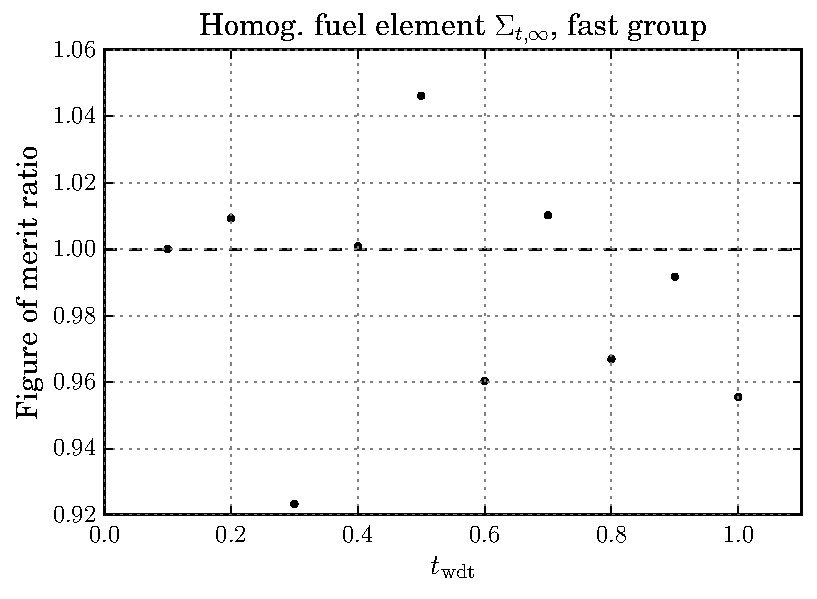
\includegraphics[scale=0.9]{images/results/homog_inf_tot_grp_comb1} \\
    (a) \\
  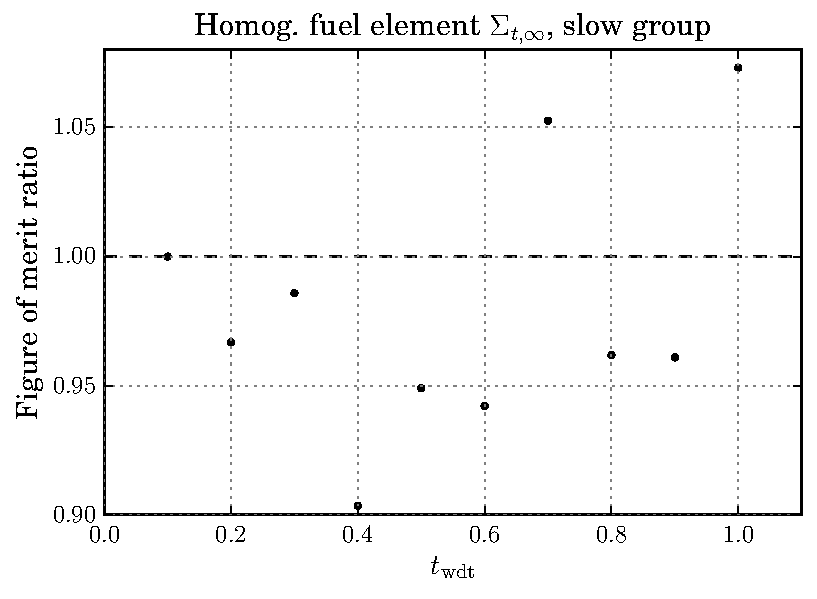
\includegraphics[scale=0.9]{images/results/homog_inf_tot_grp_comb2} \\
    (b) 
  \end{tabular}
  \caption[Figure of merit ratio of the $\Sigma_{t,\infty}$ for the
  homogeneous fuel element]{Figure of merit ratio of
    $\Sigma_{t,\infty}$ for the homogeneous fuel element vs the \gls{wdt}
    threshold for (a) fast group and (b) slow group. The group
    boundary is at $0.0625$ eV. \gls{fom} is calculated using the last
    20 data points.}
  \label{fig:homog_inf_tot}
\end{figure}

\subsection{Scattering Matrices}
\label{sec:homog_inf_sp0}

For the eleven-group case, the scattering matrices for the zeroth
moments $S_0$ is $11 \times 11$. All the tables showing the \gls{fom}
ratios for each value of the \gls{wdt} threshold are shown in
App.~\ref{sec:homog_inf_sp0_raw}. The tables are for the entry in row $g$
and column $g'$, which represents scattering from group $g'$ into
group $g$, indicated as $g' \to g$. Collapsing the groups for
comparison can not be done in this case, as the \gls{fom} is so low in
many of the matrix entries that it dominates the value of the
\gls{fom}. Instead, we have created matrix maps that show the
\gls{fom} ratios when \gls{wdt} is used. These maps are included in
App.~\ref{sec:homog_inf_sp0_mat}. 

A characteristic map is shown in Fig.~\ref{fig:homog_inf_sp0_map}, for
$t_{\mathrm{wdt}} = 0.2$. The trend we observe in these images is a
slight deviation from unity in most entries, indicating a moderate
improvement or reduction in the \gls{fom}. In only three cases did the
use of \gls{wdt} populate an entry in the matrix where the base case
did not. In each of these cases, the \gls{fom} remains very low, on
the order of $10^{-4}$. There is some improvement in the scattering
entries for group five into higher energy groups,
$\Sigma_{5 \to 1}, \Sigma_{5 \to 2},$ and $\Sigma_{5 \to 1}$. This
improvement is higher in lower values of $t_{\mathrm{wdt}}$.
\begin{figure}[hbtp]
  \centering
    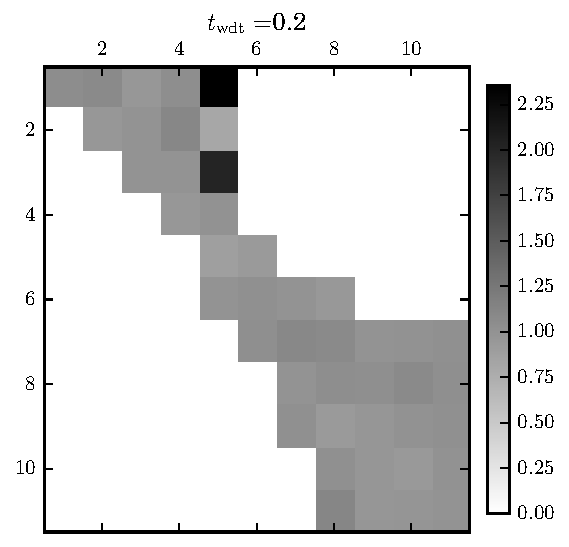
\includegraphics[scale=0.75]{images/results/matshows/homog_sp0_matshow_1}
  \caption{Matrix image for the zeroth scattering moment for the
    homogeneous fuel element for $t_{\mathrm{wdt}} = 0.2$.}
  \label{fig:homog_inf_sp0_map}
\end{figure}
\newpage
\subsection{Discussion}
\label{sec:homog_discussion}

There is no clear \gls{wdt} threshold value that creates an overall
improvement in the parameters we studied. The results of the infinite
flux show an improvement in most cases for the fast flux, and a
moderate improvement for slow flux for $0.4 \leq t_{\mathrm{wdt}} \leq
0.6$ and unity. For the infinite total cross-section, improvement in
the slow group only occurs for two values, $t_{\mathrm{wdt}} = 0.7,
1.0$. We also observe improvement in the fast group total
cross-section for $t_{\mathrm{wdt}} = 0.7$. The scattering matrices
show similar patterns for all values of the \gls{wdt} threshold. The
original use of the homogeneous fuel element by \gls{inl} is for the
development of cross-sections. Based on this intent, a threshold value
of $t_{\mathrm{wdt}} = 0.7$ will return improvements in both total
cross-section and the zeroth order scattering matrix, and near parity
with the \gls{fom} of the base case for flux. The ratios for this
parameter are summarized in Fig.~\ref{fig:homog_summary}.

\begin{figure}[hbtp]
  \centering
  \begin{tabular}{c} $t_{\mathrm{wdt}}=0.7$\\
  \begin{tabular}{lr}\toprule
    \textbf{Parameter}& $\overline{\mathbf{FOM}}$ \textbf{Ratio} \\ \midrule
    $\phi_{f, \infty}$ & 0.990465\\
    $\phi_{s, \infty}$ & 0.988462 \\
    $\Sigma_{f,t}$ & 1.010220 \\
    $\Sigma_{s,t}$ & 1.052628 \\
    \bottomrule
  \end{tabular}\\
    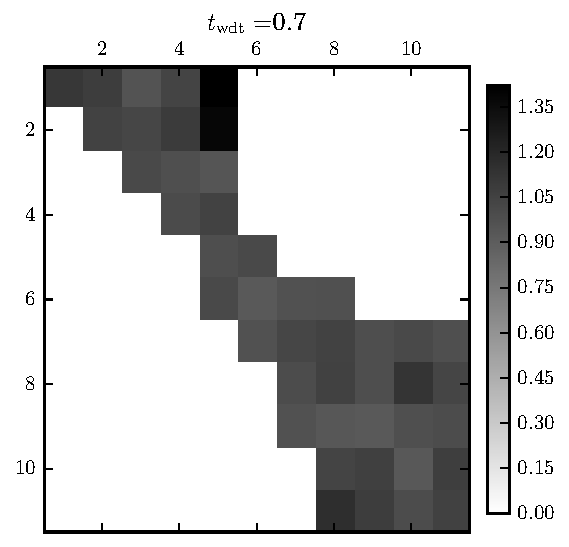
\includegraphics[scale=0.75]{images/results/matshows/homog_sp0_matshow_6}
\end{tabular}
  \caption{Summary of the data for the homogeneous fuel element for $t_{\mathrm{wdt}} = 0.7$.}
\label{fig:homog_summary}
\end{figure}



%%% Local Variables:
%%% mode: latex
%%% TeX-master: "../masters_report"
%%% End:
